\twocolumn

\chapter{Морская астронавигация\label{chap:7}}

Астрономические средства и методы навигации применяют в открытом море,
а также в прибрежных плаваниях, когда береговые ориентиры не видны или
не опознаны.

Морская астронавигация решает три основные задачи ориентирования:
определение времени, управление движением судна относительно
направления на небесное светило при плавании без компаса или
определение поправки компаса по наблюдению светила, определение
географических координат места судна по наблюдениям направлений на
светила для контроля счисления его пути.

Штурманскую квалификацию яхтенного капитана лучше всего характеризует
качество его астронавигационных обсерваций. Для решения
астронавигационных задач в полном объеме и с высокой точностью,
обеспечивающей плавание в открытом море, на яхте необходимо иметь:
транзисторный радиоприемник для приема радиосигналов времени,
навигационный секстан, хорошие влагозащищенные часы (лучше всего
электронные или кварцевые, со стрелочной индикацией),
микрокалькулятор, способный вычислять тригонометрические
функции\footnote{Подойдет любой современный микрокалькулятор, включая
  те, что есть в современных смартфонах. Лучше иметь отдельное
  устройство, что бы не зависеть от заряда аккумуляторов смартфона.
  Рекомендуется, например, калькулятор серии CASIO FX-82. Примеры,
  которые есть в книге приведены для этой модели калькулятора}, или
таблицы <<Высоты и азимуты светил (ВАС-58)>>, изданные ГУНиО, Морской
Астрономический Ежегодник (МАЕ) или другое пособие для вычисления
координат светил.

Если какой-либо из упомянутых инструментов или пособий на яхте
отсутствует, снижается точность и частота обсерваций
астронавигационного ориентирования.

\section{Небесные ориентиры, их координаты и видимые движения\label{sec:7-1}}

Ориентирами в астронавигации являются небесные светила: звезды,
Солнце, Луна и наиболее яркие планеты (Венера, Марс, Юпитер, Сатурн).

\textbf{Навигационные звезды.} Навигационными называют наиболее яркие
звезды, которые наблюдают для ориентирования (основные перечислены в
приложении~\ref{app:4},~\textit{а}). Звезды опознают по их
расположению в созвездии \--- в характерной фигуре, образованной
группой соседних звезд на небосводе, а также по их видимому блеску.
Блеск звезд сравнивают с помощью условных чисел \--- звездных величин,
шкала которых имеет вид:

\begin{center}
  \small
  \begin{tabular}[c]{cccccccc}
    \ldots & $-2$ & $-1$ & 0 & $+1$ & $+2$ & $+3$ & \ldots \\
    \multicolumn{3}{c}{Блеск сильнее} & & \multicolumn{4}{c}{Блеск слабее} \\
    \multicolumn{3}{c}{$\longleftarrow$} & & \multicolumn{4}{c}{$\longrightarrow$} 
  \end{tabular}
\end{center}

\begin{figure*}[!htb]
  \centering{}
  \includegraphics[width=0.8\linewidth]{0087P}
  \caption{Ориентирование по направлению на север, во времени и по
    широте места яхты по наблюдению за созвездиями северного неба}
  \label{fig:87}
\end{figure*}

Блеск $m=0$ присвоен самой яркой звезде летнего неба \starName{Веге}
(\alphaStar{Лиры}). Почти такой же яркости \starName{Арктур}
(\alphaStar{Волопаса}). \starName{Альтаир} (\alphaStar{Орла}) имеет
$m = 1$, и она считается в 2,5 раза слабее по блеску чем
\starName{Вега}; \starName{Дубхе} ($\upalpha$~Большой Медведицы) имеет
блеск $m = 2,0$, и она видна слабее \starName{Веги} в
$2,5 \cdot 2,5 \approx 6$ раз. Буквой $\upalpha$ обычно обозначается
самая яркая звезда того созвездия, название которого указано.

Приступая к самостоятельному изучению звездного неба, определяют по
компасу направление на точку севера $N$ (рис.~\ris{87}). Над точкой
$N$ в угловом расстоянии $h$, равном географической широте места
наблюдений $\varphi_N$, расположена \starName{Полярная}
($\upalpha$~Малой Медведицы). Приближенно можно полагать, что с
\starName{Полярной} совпадает точка $P_N$ \--- Северный полюс
мира. \textbf{Угол между плоскостью горизонта и направлением на наблюдаемое
светило называется высотой светила.\index{высота светила}} Высота
\starName{Полярной} приближенно равна географической широте места
яхты.

Земная атмосфера наблюдается нами в форме приплюснутого над головой
<<небесного свода>>. Это искажает глазомерно измеряемые высоты:
наблюдаемая невооруженным глазом высота светила обычно представляется
на 15\otdo 20\gr больше истинной высоты.

Направление на наблюдаемое светило определяет его истинный пеленг \IP;
в астронавигации эту координату часто называют \textbf{круговым
  азимутом} и обозначают $A_K$. При вычислениях удобно измерять азимут
<<вполкруга>>: в северной широте \--- от точки севера $N$ по
горизонту, в направлении точек востока или запада, в пределах 0\otdo
180\gr. \textbf{Полукруговой азимут} обозначают \AP и записывают в
форме, например, $\AP = N68\gr\Ost$ . Если компас не имеет
пеленгатора, то \IP светила можно найти, заметив в один и тот же
момент курсовой угол светила и курс яхты: $\IP = \IK \pm \KU$ (знак
ставится в зависимости от наименования борта: ($-$) соответствует
левому борту). \IP \starName{Полярной} близок к 0\gr, поэтому \IK приближенно
равен \KU \starName{Полярной}. На рис.~\ris{87}  \starName{Кастор}
($\upalpha$~Близнецов) видна по направлению $\IP^* = 68\gr$ на высоте
$h^* = 25\gr$, если наблюдения ведутся на широте
$\varphi \approx 44\gr N$ (Севастополь, Владивосток).

Высота и азимут (горизонтальные координаты) вполне определяют
положение видимого места светила, поскольку их отсчитывают от
горизонта (высота), либо измеряют по горизонту (азимут). Высоту можно
измерить с помощью секстана или астролябии, круговой азимут \--- с
помощью компаса и пеленгатора.

Опознав \starName{Полярную}, легко найти созвездие Большой Медведицы
(Большой Ковш) и <<девичью грудь>> Кассиопеи \--- оба эти созвездия
расположены на небосводе в угловом удалении 30\otdo 40\gr по обе
стороны от \starName{Полярной}; при наблюдениях на наших морях они
всегда расположены над горизонтом. Большую Медведицу легко запомнить и
быстро отыскать на небе, относительно нее просто опознать другие
созвездия и навигационные звезды:

\begin{itemize}
\item по направлению от $\upbeta$ на $\upalpha$~Большой Медведицы (и в
  удалении, равном пяти расстояниям $\upbeta - \upalpha$) находится
  \starName{Полярная} и <<Малый Ковш>> созвездия Малой Медведицы;
\item по направлению $\upgamma$ Б.М. \--- \starName{Полярная} и на
  таком же расстоянии от \starName{Полярной} находится Кассиопея;
\item по направлению $\upgamma$ \--- $\updelta$ Б.М. видны созвездия
  Лиры и Лебедя, входящие вместе с созвездием Орла в <<летний
  треугольник>>;
\item по направлению $\updelta$ \--- $\upalpha$ Б.М. виден Возничий.
\end{itemize}

Для изучения других созвездий служит карта звездного неба, прилагаемая к МАЕ.

На рис.~\ris{88} изображен земной шар и показано географическое место
яхты $M$, имеющее координаты $\varphi_N$ и $\lambda_\Ost$. Затем
произвольным радиусом из центра Земли описана вспомогательная небесная
сфера, и на ней показано \textbf{видимое место светила} $\sigma'$ как
точка пересечения поверхности сферы и пришедшего от очень удаленного
светила луча света; аналогичная точка на поверхности Земли называется
\textbf{географическим местом светила} $\sigma$ (или ГМС).

\begin{figure}[!htb]
  \centering{}
  \includegraphics[width=\linewidth]{0088P}
  \caption{Географические и экваториальные координаты, определяющие
    положение географических и видимых мест светил}
  \label{fig:88}
\end{figure}

Если через географическое место светила а провести меридиан
$P_N \sigma P_S$, a через видимое место светила провести аналогичный
небесный меридиан $P_N \sigma' P_S$, то нетрудно определить положение
географического и видимого места светила в географической системе
координат:

\begin{itemize}
\item широте ГМС $\varphi^*$ на сфере соответствует дуга меридиана
  $\delta$, в астронавигации ее называют \textbf{склонением светила};
  склонение измеряют так же, как и географическую широту; при плавании
  в северном полушарии северное склонение считается положительной
  величиной, а южное \--- отрицательной;
\item долготе ГМС $\lambda^*$ на сфере соответствует дуга экватора
  $\cidx{E}{ГР} E^* = \cidx{t}{ГР}$, в астронавигации ее называют
  \textbf{гринвичским часовым углом светила} и измеряют аналогично
  географической долготе или же в круговом счете \--- от небесного
  гринвичского меридиана по экватору всегда в сторону запада от 0 до
  360\gr.
\end{itemize}

Положение меридиана видимого места светила на небесной сфере можно
определить не только от гринвичского меридиана. Из рис.~\ris{88}
видно, что дуга экватора от местного небесного меридиана до меридиана
видимого места светила измеряет \textbf{местный часовой угол} $t_M$
(его отсчитывают аналогично гринвичскому, но за начало отсчета принята
точка $E$ экватора на полуденной части $P_N E P_S$ местного меридиана). Местный
часовой угол отличается от гринвичского на величину долготы места
яхты:

\begin{equation}
  t_M^W = \cidx{t}{ГР}^W \pm \lambda_W^\Ost
\end{equation}

где восточная долгота прибавляется к $\cidx{t}{ГР}^W$ кругового счета,
а западная \--- вычитается.

Часовой угол светила можно также отсчитать круговым счетом от той
точки экватора, в которой Солнце расположено на небосводе в день
наступления весны \--- 21 марта. Эта точка называется \textbf{точкой
  весны (точкой Овна)} и обозначается \Aries. Отсчитанный от точки
Овна часовой угол называется \textbf{звездным углом} (в МАЕ он назван
\textbf{звездным дополнением}) и обозначается $\uptau^*$.

Величина $360\gr - \uptau^* = \alpha$ называется \textbf{прямым
  восхождением} и отсчитывается противоположно звездному углу. Прямые
восхождения получают из МАЕ для указания видимых мест планет, Луны и
Солнца.

Координаты $\delta$, $t_M$, \cidx{t}{ГР}, $\uptau^*$, $\alpha$ вполне
определяют положение на небесной сфере и на звездной карте небесной
параллели светила (склонение) и небесного меридиана светила (одна из
величин: $t_M$, \cidx{t}{ГР}, или $\uptau^*$, $\alpha$). Эти координаты
называют экваториальными, на яхте их вычисляют по МАЕ или другому
пособию на момент наблюдений светила.

Из рис.~\ris{88} видно, что в любой момент:

\begin{equation}
  t_M = \tauAries + \uptau^* 
\end{equation}

Часовой угол точки Овна \tauAries называют \textbf{звездным временем}. На
звездной карте очень близко к меридиану точки Овна расположена \starName{Кафф}
($\upbeta$~Кассиопеи), а на противолежащем меридиане расположена
\starName{Фекда} ($\upgamma$~Большой Медведицы). Значит, по часовому углу
\starName{Кафф} непосредственно из наблюдений можно узнать звездное время,
а часовой угол \starName{Фекда} отличается от звездного времени на 180\gr
(тогда $\tauAries = t_M^* - 180\gr$). Для оценки на небосводе часовых
углов этих звезд полезно помнить, что угловое расстояние на реальном
небосводе между звездами $\upbeta$ \--- $\upvarepsilon$~Кассиопеи
приближенно равно $15\gr = 1\thr$, а между звездами $\upalpha$ \---
$\upeta$~Большой Медведицы оно равно $25\gr = 1,7\thr$. На рис. 87:
$\tauAries = 30\gr$.

Если небесный экватор разделить на 24 части, то каждая часть будет
равна 15\gr. Ее называют \textbf{часом}; поделив час на 60 частей,
получают \textbf{минуту} (4\tmin = 1\gr и 1\tmin = 15 дуговых минут),
поделив минуту на 60 частей, получают \textbf{секунду} (4\tsec = $1'$
и 1\tsec = $0,25'$). В часовой мере измеряют время и, когда это удобно
для практики, часовые углы.

\begin{small}
  Применительно к рис.~\ris{88} географические и экваториальные координаты записывают так:
  \begin{itemize}
  \item Место яхты: $\varphi = 44\gr N$, $\lambda = 65\gr \Ost$.
  \item Географическое место светила: $\varphi^* = 50\gr N, \lambda^* = 35\gr W$.
  \item Видимое место светила: $\delta = 50\gr N$, $\cidx{t}{ГР} = 35\gr W$ или $t_M = \cidx{t}{ГР}+ \lambda^\Ost = 35\gr + 65\gr = 100\gr W$;
  \item Звездное время: $\tauAries = 28\gr$ или \hhmm{1}{52};
  \item Звездный угол (звездное дополнение): $\uptau^* = 72\gr$;
  \item Прямое восхождение: $\alpha = 288\gr$.
  \end{itemize}
\end{small}

На рис.~\ris{87} $\tauAries = 30\gr = 2\thr$, так как
$\upbeta$~Кассиопеи наблюдается западнее полуденной части местного
небесного меридиана, a $\upgamma$~Большой Медведицы \--- восточнее
полуночной части местного меридиана. Звезда $\upalpha$~Лиры имеет
$t_M = 110\gr W$, a звезда $\upalpha$~Близнецов имеет часовой угол
$t_M = 85\gr$.

Экваториальные координаты навигационных звезд, наблюдения которых чаще
всего встречаются в астронавигационных задачах, даны в
приложении~\ref{app:4}, \textit{а}, воспроизводящем с небольшими
дополнениями сведения из МАЕ на високосный, 1980~г. Звездная карта МАЕ
также основана на экваториальных координатах; в условиях яхтенного
плавания она заменяет звездный глобус. В левой верхней части карты
дана северная полярная часть звездного неба, а в правой верхней части
\--- его южная полярная часть. В обоих случаях даны звезды со
склонениями от 30 до 90\gr, меридианы имеют величины звездных углов
$\uptau^*$ через 30\gr. Экваториальная область между параллелями
$\pm 23,5\gr$ дана внизу; здесь по верхней рамке отсчитывают прямые
восхождения и звездное время, а по нижней \-- звездные углы (звездные
дополнения) $\uptau^*$. Правая стрелка показывает направление видимого
суточного движения светил; слева внизу указаны широты, при которых
данная параллель касается горизонта в точке юга.

\textbf{Пользование звездной картой.} Для опознания звезд карту
необходимо сориентировать по широте места, направлению местного
меридиана наблюдателя и времени наблюдений.

Наметив по часам момент \cidx{T}{С} начала предстоящих наблюдений
звезд (о системе счета времени на яхте см. раздел~\ref{sec:7-2} и
рис.~\ris{90}) по схеме, данной в примере~1, прежде всего
заблаговременно вычисляют звездное время в момент
\cidx{T}{С}. Точность вычислений с погрешностью до получаса достаточна
для работы с картой.

\begin{table*}[!tb]
  \small
  \centering
  Таблица к примеру 1: \\
  \begin{tabular}{p{0.4\textwidth}|c|c}
    \toprule
    Величина, действие & Усл. обозначения & Решение \\
    \midrule
    1.~Cтандартное время срока наблюдений & \cidx{T}{С} & 12 февраля 20,5\thr \\
    \midrule
    2.~Разница между стандартным и теоретическим поясным временем по рис.~\ris{90} & $\Delta \cidx{T}{С}$ & $-1\thr$ \\
    \midrule
    3.~Поясное время (приближенное меридианное время) & $\TNo \approx \cidx{T}{M}$ & 12 февраля 19,5\thr \\
    \midrule
    4.~Вспомогательная величина из прилож.\ref{app:4}, \textit{в} на 12 февраля & $R$ & $-14,5\thr$ \\
    \midrule
    5.~Звездное время на местном меридиане & \tauAries & 5\thr \\
    \bottomrule
  \end{tabular}
\end{table*}

\begin{small}
  \textbf{Пример 1.} Намечены наблюдения звездного неба в Ленинграде
  (широта места $\varphi = 60\gr N$) 12 февраля около
  $\cidx{T}{С} = \hhmm{20}{20}$.  Вычислить звездное время на
  начало наблюдений для работы с картой звездного неба\footnote{Все последующие
  примеры даны по такой же схеме.}.
  
  \textbf{Пояснения:}
  
  \begin{enumerate}
  \item Если при выполнении пп. 1\--3 получается отрицательная величина,
    то надо увеличить \cidx{T}{С} на 24\thr; после вычитания \cidx{T}{С}
    получится $T_\mathNo$ на предыдущую календарную дату.
  \item В нашей стране: с 1 октября по 1 апреля
    $\Delta \cidx{T}{С}=-1\thr$, а с 1 апреля по 1 октября
    $\Delta \cidx{T}{С} = -2\thr$. В других случаях $\Delta \cidx{T}{С}$
    есть разница между стандартным и поясным временем (рис.~\ris{90}).
  \item Разница между меридианным $T_M$ и поясным $T_\mathNo$ не
    превышает 30\tmin.
  \item Вспомогательная величина $R$ выбирается по заданной дате
    наблюдений из прилож.~\ref{app:4}, \textit{в} с округлением до
    получаса.
  \item Получается всегда действием вычитания:
    $\text{п}.~5 = \text{п}.~3 - \text{п}.~4$; при необходимости
    увеличить $T_\mathNo$ на 24\thr.
  \end{enumerate}
\end{small}

Для работы на карте звездное время \tauAries переводят в градусную
меру по табл. приложения~\ref{app:4}, \textit{б} либо в уме умножением
на 15\gr: $\tauAries = 5 \cdot 15\gr = 75\gr$.

Далее на карте по шкале прямых восхождений следует найти меридиан
75\gr и точку его пересечения с экватором $E$ \--- она называется
\textbf{полуденной точкой}. По широте места $\varphi = 60\gr N$
находят ту параллель, которая касается горизонта в точке юга \--- при
этом пользуются шкалой слева внизу карты. Звезды, расположенные южнее
этой параллели, в данной северной широте никогда не видны.

Выйдя на наблюдения, прежде всего находят основные направления
(ориентируясь по \starName{Полярной} или по компасу): на север $N$, на
восток $\Ost$, на юг $S$, и на запад $W$. Затем определяют положение
небесного местного меридиана: он проходит от $N$ через Северный полюс
мира $P_N$, далее через точку над головой наблюдателя $Z$ (зенит) и
через точку $S$. Карту размещают так чтобы полуденная точка $E$ была
над точкой юга $S$ и вычисленный меридиан 75\gr совпал с направлением
местного меридиана; при этом высота точки $E$ должна быть равна
$90\gr - \varphi = 30\gr S$.

Вблизи местного меридиана, несколько восточнее точки юга, на высоте от
20 до 40\gr (по условию примера 1) опознают созвездие Ориона; на
продолжении трехзвездной дуги <<пояса Ориона>> вправо и вверх
располагаем \starName{Альдебаран} ($\upalpha$~Тельца). Продолжив эту
же дугу влево и вниз, найдем самую яркую звезду зимнего неба
\starName{Сириус} ($\upalpha$~Большого Пса). Непосредственно над
головой наблюдателя проходят те светила, у которых склонение равно
широте места наблюдений; близко к зениту разместилось созвездие
Возничего.

На карте звездного неба северная полусфера дана с оцифровкой
меридианов величинами $\uptau^*$. Вычислив звездный угол точки $E$
($\uptau^E = 360\gr - t^v = 360\gr - 75\gr = 285\gr$), найдем
меридиан, проходящий через \starName{Полярную} и зенит. Теперь над
точкой севера опознаем звезды созвездия Геркулеса. На высоте 60\gr
располагается \starName{Полярная}, Кассиопея видна левее и выше
\starName{Полярной} (часовой угол \starName{Кафф} равен
$t_M = 75\gr = 5\thr \Ost$. Большая Медведица видна правее и ниже
\starName{Полярной}, часовой угол \starName{Фекда}
$t_M = 255\gr W = 105\gr \Ost$.

В результате вращения Земли вокруг своей оси наблюдается видимое
вращение небосвода с востока на запад: если смотреть на север, то
видимое движение светил происходит вокруг \starName{Полярной} против
хода часовой стрелки (см. рис.~\ris{87}). Если же смотреть на юг, то
видимое движение светил происходит по ходу часовой стрелки. В нашем
примере созвездие Ориона перемещается слева направо \--- в сторону
запада. Скорость видимого суточного движения светил составляет около
15\gr в час, поэтому экваториальное созвездие Ориона зайдет примерно
спустя 6\thr после его прохождения через меридиан места наблюдений
(после кульминации). Это произойдет в
$\cidx{T}{С} \approx 20\thr + 6\thr = 26\thr - 24\thr = 2\thr$ 13
февраля.

Перед плаванием полезно потренироваться в опознании звезд на местности
или с помощью карты звездного неба.

\textbf{Видимые движения светил Солнечной системы.} Кроме видимого
суточного движения, в котором участвуют все светила, существует
собственное перемещение по небесной сфере светил Солнечной системы
(Солнца, планет, Луны) с разными периодами. В результате этого
перемещения они по-разному видны на небосводе в различные календарные
даты и периодически появляются в различных участках звездного неба.

В течение года Земля совершает один оборот по орбите вокруг Солнца
поэтому Солнце имеет собственное годовое движение на фоне
созвездий. Путь Солнца среди звезд, показанный пунктиром на карте
звездного неба, называется \textbf{эклиптикой}: Солнце перемещается
среди созвездий зодиакального пояса (<<круга животных>>), проходя
последовательно с марта по февраль созвездия Рыбы (\Pisces), Овна
(\Aries), Тельца (\Taurus), Близнецов (\Gemini), Рак (\Cancer), Льва
(\Leo), Девы (\Virgo), Весов (\Libra), Скорпиона (\Scorpio), Стрельца
(\Sagittarius), Козерога (\Capricorn), Водолея (\Aquarius). Скорость
этого перемещения составляет около 1\gr за сутки или $30\gr = 2\thr$
за месяц, поэтому картина звездного неба в данном месте и в данный час
суток спустя месяц будет наблюдаться на 2 часа раньше, спустя 15 суток
\--- на 1 час раньше и т.\=,п. В полночь на юге располагаются
созвездия, отстоящие от Солнца по экватору на $180\gr = 12\thr$.
Например, 22 июня прямое восхождение Солнца $\alpha = 90\gr = 6\thr$ и
в местную полночь на юге будут видны созвездия Змееносца и Лиры
(см. приложение~\ref{app:4}, \textit{б}).

Из девяти планет Солнечной системы для целей навигации наблюдают
только Венеру (\Venus), Марс (\Mars), Юпитер (\Jupiter) и Сатурн
(\Saturn). Блеск планет бывает очень большим (иногда Венера видна днем
невооруженным глазом), но изменяется в зависимости от взаимного
расположения планеты, Земли (\Earth) и Солнца (\Sun) (конфигурации),
смена которых происходит с периодом от 1 до 2 лет. Планеты всегда
наблюдаются в пределах зодиакального пояса, недалеко от
эклиптики. Сведения об их положении на небосводе на каждый день и
характеристику их видимости можно получить из МАЕ или из
Астрономического календаря, который ежегодно выпускает издательство
<<Наука>>.

Появление планеты может значительно исказить вид созвездия и
затруднить его опознание, планета может быть перепутана с
навигационной звездой. Поэтому необходимо нанести видимые места планет
на звездную карту для намеченного срока плавания (по указанным в МАЕ
или Астрономическом календаре величинам $\alpha$ и $\delta$).

\begin{figure*}[!htb]
  \centering{}
  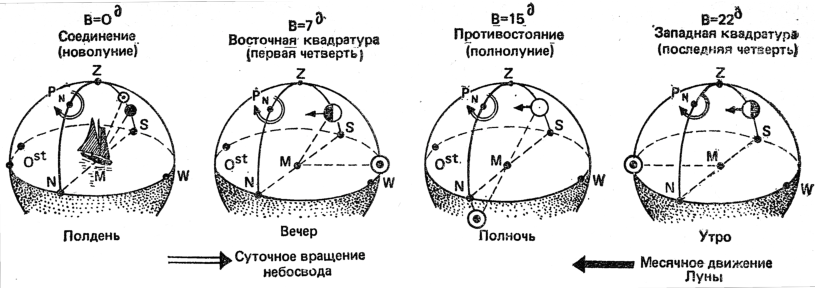
\includegraphics[width=0.8\linewidth]{0089P}
  \caption{Условия наблюдений Луны и лунная освещенность зависят от возраста Луны и широты места яхты}
  \label{fig:89}
\end{figure*}

Венеру следует наносить не реже чем каждую неделю, Марс \--- через две
недели, Юпитер и Сатурн \--- через месяц.

Луна (\Moon) также перемещается среди созвездий зодиакального пояса и
имеет собственное движение с запада на восток примерно на величину
своего видимого диска за каждый час. За сутки это смещение составляет
около $13\gr \approx 50\tmin$. Вид Луны на небе называется
\textbf{фазой}, которая зависит от ее возраста.

\textbf{Возраст Луны} выражается в сутках и указывает количество
суток, прошедших после того дня, когда Луна и Солнце были на одном
небесном меридиане (рис.~\ris{89}). При соединении Луны и Солнца
возраст $\mcyr{В} = 0$, Луна обращена к нам неосвещенной стороной и не
наблюдается на небе: эта фаза называется новолунием. В новолуние Луна
проходит над точкой юга одновременно с Солнцем, возраст Луны на любую
дату подсчитывают по формуле:

\begin{equation}
  \mcyr{В} = \mcyr{Д} + \mcyr{М} + \mcyr{Л} \ , \label{eq:58}
\end{equation}

где: \mcyr{Д} \--- календарная дата; \mcyr{М} \--- номер месяца в
году; \mcyr{Л} \--- лунное число (в 2023~г. оно равно 7 и затем каждый
год увеличивается на 11).

Например, если $\cidx{\mcyr{Л}}{1982} = 2$, 8~мая 1984~г.:
$\cidx{\mcyr{Л}}{1984} = 2 + 11 \cdot 2 = 24$; $\mcyr{Д} = 8$;
$\mcyr{М} = 5$. $\mcyr{В} = 37 - 30 = 7\tday$.

Период смены фаз равен $29,5\tday = 30\tday$ поэтому его величину
после расчета при необходимости отбрасывают.

При $\mcyr{В} = 7\tday$ Луна расположена к востоку от Солнца и видна в
первой четверти (молодая Луна); она восходит около полудня, во вторую
половину дня видна вместе с Солнцем над горизонтом, вечером освещает
юго-западную сторону горизонта и заходит около полуночи.

При $\mcyr{В} = 15\tday$ Луна и Солнце расположены на противоположных
меридианах (в противостоянии, \textit{сизигии}) наблюдается
полнолуние. Луна восходит вечером и до утра освещает ночной горизонт;
здесь лунная освещенность максимальна.

При $\mcyr{В} = 22\tday$ Луна расположена западу от Солнца и видна в
последней четверти (старая Луна), она восходит около полуночи, в
первую половину дня вместе с Солнцем видна над горизонтом и заходит
около полудня. Спустя неделю начнется новый период смены фаз Луны.

В плавании Луну наблюдают и днем, и ночью. Ее место на звездной карте
отмечают непосредственно на намеченный срок наблюдений (по $\alpha$ и
$\delta$, указанным в Астрономическом календаре или МАЕ, при этом в
МАЕ приходится находить
$\alpha^{\text{\Moon}} = \cidx{t}{ГР}^{\text{\Aries}} -
\cidx{t}{ГР}^{\text{\Moon}}$). Лунная освещенность в значительной
степени зависит от фазы Луны и ее высоты над горизонтом; последняя же
в течение месяца изменяется вследствие быстрого и большого изменения
склонения Луны.

Описанная картина верна для наблюдений в  $\varphi > 23,5\gr N$.

\section{Ориентирование во времени\label{sec:7-2}}

Время на яхте необходимо знать с различной точностью. Если для ведения
навигационной прокладки требуется знать время с погрешностью не более
минуты, то для астронавигационного определения долготы места яхты
нужно знать его с погрешностью до 1 секунды, так как здесь ошибка во
времени равна ошибке в найденной долготе ($4\tmin = 1\gr$,
$1\tmin = 15'$, $4\tsec = 1'$ и т.\=,д.).

Часы на яхте в автономном плавании могут быть установлены по
разнообразным системам счета времени. Решение об этом принимает
капитан \--- он должен позаботиться о том, чтобы время на яхте
измерялось непрерывно и достаточно точно. Кроме того, при заходе в
порты счет времени должен быть согласован со счетом времени, принятым
в пункте захода. Потеря информации о времени при плавании в открытом
море считается чрезвычайным происшествием, чреватым угрозой
безопасности плавания.

\begin{figure*}[!htb]
  \centering{}
  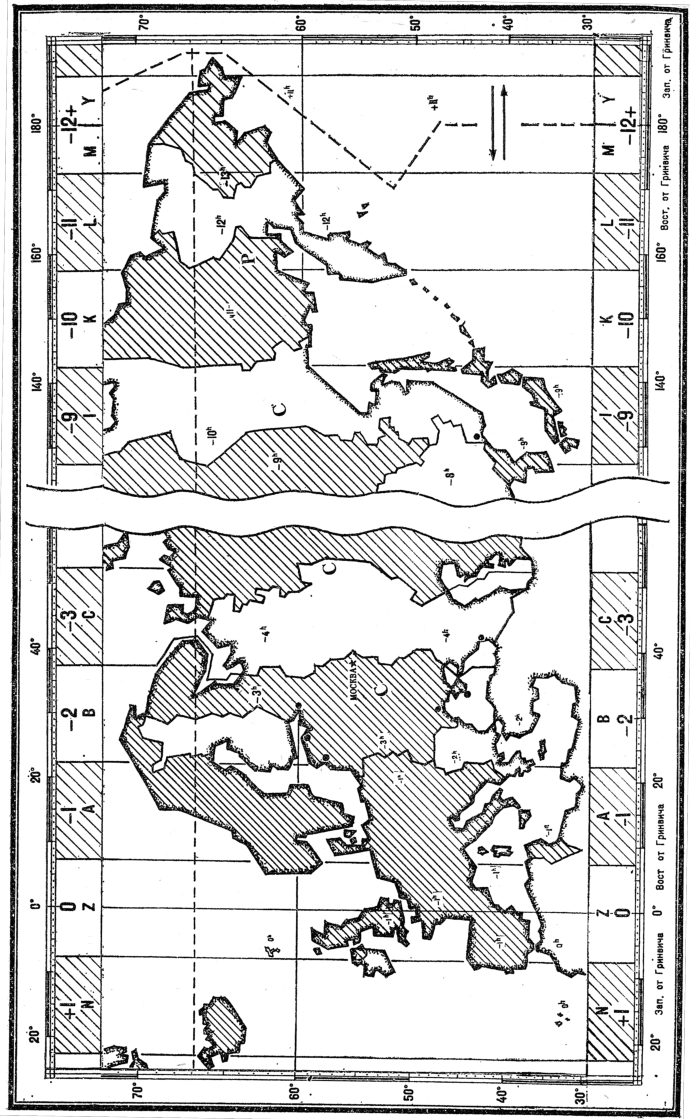
\includegraphics[width=0.8\linewidth]{0090P}
  \caption{Зимнее стандартное время на територии СССР. Знаки у номеров часовых поясов даны для перехода ко всемирному времени}
  \label{fig:90}
\end{figure*}

\textbf{Системы измерения времени.} Принятые в различных странах
системы измерения времени можно узнать по карте часовых поясов (карта
\No 90080, издания ГУНиО МО СССР; такого же назначения карты
публикуются в географических и морских атласах). Часть карты часовых
поясов для европейских государств, а также для европейских и
дальневосточных районов Советского Союза приведена на
рис.~\ris{90}. Здесь показано стандартное время, система счета
которого определена постановлением (декретом) правительства данной
страны и является обязательной на всей ее территории. В большинстве
стран в основе стандартного времени (обозначается \cidx{T}{С}) лежит система
счета по часовым поясам.

Повседневная жизнь организована по движению Солнца, и наши часы
показывают солнечное время, следят за видимым суточным движением
Солнца (рис.~\ris{91}). \textbf{Солнечное время} измеряют от полуночи
\--- с момента прохождения Солнцем полуночной части местного меридиана
$P_NNQP_S$ наблюдателя $M$; оно называется \textbf{меридианным}, или
\textbf{местным}, солнечным временем (обозначается $\TSun_M$).
 
\begin{figure}[!htb]
  \centering{}
  \includegraphics[width=\linewidth]{0091P}
  \caption{Солнечное время по наблюденному часовому углу Солнца}
  \label{fig:91}
\end{figure}

Часовые углы Солнца измеряют от полуденной точки $E$ экватора, поэтому
до полудня местное солнечное время равно
$\TSun_M = 12\thr - \tSun_\Ost$ и после полудня
$\TSun_M = 12\thr + \tSun_W$. Если с помощью компаса определить
положение \textbf{полуденной линии} $S-N$ на местности, затем глазомерно
оценить положение точки $E$ на небесном меридиане (по величине угла
$90\gr - \varphi$) и положение небесного экватора ($\Ost EW$), а после
этого \--- величину наблюдаемого восточного или западного часового
угла Солнца, то по показанным формулам получим приближенную
ориентировку во времени текущих суток.

\textbf{Сутки} \--- это длительность одного оборота Земли вокруг своей
оси, измеренная относительно направления на Солнце. Они являются
основной единицей измерения времени. Как уже было сказано
в~\ref{sec:7-1}, сутки делят на часы, минуты и секунды.


\begin{figure*}[!htb]
  \begin{minipage}[b]{0.49\textwidth}
    \centering
    \includegraphics[width=\linewidth]{0092-1P}
  \end{minipage}
  \hfil\hfil
  \begin{minipage}[b]{0.49\textwidth}
    \centering
    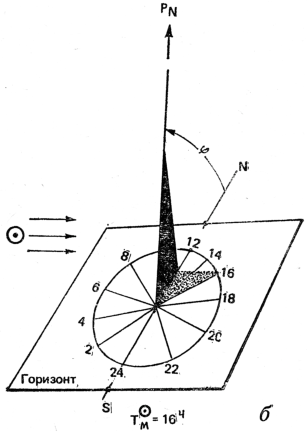
\includegraphics[width=\linewidth]{0092-2P}
  \end{minipage}
  \caption{Солнечные часы}
  \label{fig:92}
  \small
  \centering{}
  \textit{а} \--- экваториальные; \textit{б} \--- горизонтальные
\end{figure*}


Ход местного солнечного времени воспроизводят солнечные часы,
устройство которых показано на рис.~\ris{92}. Эти часы можно
изготовить самостоятельно. \textbf{Экваториальные солнечные часы}
устанавливают отметкой 12\thr на точку севера $N$ и линию 24\thr \---
12\thr с возможно большей точностью совмещают с направлением
полуденной линии $S-N$. Их циферблат имеет равномерную шкалу
($15\gr = 1\thr$) и располагается под углом $90\gr - \varphi$ к
плоскости горизонта. Измеряемый момент времени отмечает на циферблате
тень от штока, установленного в центре циферблата и перпендикулярно к
нему. Точность такого измерения зависит от качества изготовления
часов, масштаба делений циферблата (ошибка в отсчете момента по
циферблату на 1\gr даст ошибку во времени на 4\tmin, точности
установки основания часов в плоскости горизонта и относительно
полуденной линии $S-N$.

Циферблат \textbf{горизонтальных солнечных часов} устанавливается в
плоскости горизонта, и его линия 24\thr \--- 12\thr совмещается с
полуденной линией $S-N$. Шкала циферблата этих часов неравномерна, ее
вычисляют по формуле (\ref{eq:59}) с помощью микрокалькулятора или по
таблицам натуральных величин тригонометрических функций:

\begin{equation}
  \tg x = \sin \varphi \tg t \label{eq:59}
\end{equation}

где $\varphi$ \--- широта места, $t$ \--- интервал времени от полудня,
$x$ \--- угол между полуденной линией и отметкой часа,
соответствующего $t$.

Теневая пластина устанавливается в плоскости местного меридиана, и ее
верхний срез должен быть направлен на Северный полюс мира под углом
$\varphi$ к горизонту. Кроме отмеченных причин погрешность измерения
времени по горизонтальным часам зависит от широты места и времени
суток, она больше вблизи полудня и в малых широтах.

В морских условиях применению солнечных часов мешает качка, их надо
устанавливать на азимутальном круге котелка магнитного
компаса. Солнечные часы применяются в различных упрощенных
ориентаторах для определения долготы места и момента наступления
полудня\footnote{См. <<Круйзерфикс>> \--- заменитель
  секстана. <<Катера и яхты>>, \No 5 (75), 1978~г.}. В момент полудня
тень от вертикально установленного штока имеет наименьшую длину и
располагается по линии от $S$ к $N$ (если $\varphi > 23,5\gr N$).

Измерив время по солнечным часам и сравнив его с показанием времени по
механическим или электронным часам, обнаружим значительную разницу
\--- иногда до 2\thr и даже более. Причина \--- в особенности
конструкции наших обычных часов и принятого стандартного времени для
их установки.

Глядя на рис.~\ris{91}, спроектируйте со стороны $P_N$ изображенное на
нем северное полушарие небесной сферы на плоскость экватора: в этой
проекции полюс $P_N$ будет в центре экватора, а всe меридианы
изобразятся прямыми линиями и их движение будет происходить с востока
на запад, по часовой стрелке. Циферблат наших часов есть проекция
северного полушария сферы на плоскость экватора, часовая стрелка есть
меридиан Солнца, а ее движение воспроизводит вращение Земли, точнее
говоря \--- суточное вращение неба. Остается пояснить, что чаще всего
циферблаты часов ради удобства от счета делят не на 24\thr, а на
12\thr и скорость вращения часовой стрелки увеличивают в два
раза. Поэтому во второй половине суток для определения времени по
такому циферблату приходится мысленно увеличивать отсчеты на
12\thr. Кроме того, стрелка часов движется всегда равномерно, а
истинное Солнце изменяет свое положение на небосводе в течение года не
вполне равномерно. Поэтому воспроизводимое обычными часами равномерное
время (его называют \textbf{средним временем} и обозначают $T$) на
несколько минут отличается от солнечного времени $\TSun_M$ по
солнечным часам.

Время, измеренное от полуночной части местного меридиана в средних
единицах (т.\=,е. средней за год длительностью суток, часа, минуты,
секунды), называется \textbf{меридианным}, или \textbf{местным},
средним временем и обозначается $T_M$. Можно сказать, что наши часы
воспроизводят движение условного равномерно идущего <<среднего
Солнца>>.

Угол $\eta$, который в данный день образуется между меридианами
среднего Солнца и истинного Солнца, называется \textbf{уравнением
  времени}. Чтобы от показания времени $\TSun_M$ по солнечным часам
перейти к показанию среднего времени $T_M$, надо величине $\TSun_M$
придать уравнение времени со знаком, указанным в
приложении~\ref{app:4},~\textit{в}. Например, 24 июля по приложению
$\eta = +6,4\tmin$, и если по солнечным часам в полдень всегда
$T_M = 12\thr\ 00\tmin$, то по нашим <<средним>> часам 24 июля время
наступления полудня будет $T_M = 12\thr\ 06,4\tmin$ меридианного
времени.

При \textbf{поясном счете среднего времени} (см. рис.~\ris{90}) весь земной шар
делят на часовые пояса, теоретически имеющие протяженность
$15\gr = 1\thr$ по долготе. Эти пояса показаны на карте возле ее
верхней и нижней рамок: они имеют буквенные и цифровые обозначения. В
пределах часового пояса во всех его местах часы устанавливают по
одному и тому же времени \--- по меридианному среднему времени
центрального (осевого) меридиана данного пояса. Например, в поясе
$Z(0)$ \--- по времени Гринвичского меридиана ($\lambda = 0\gr$), в поясе
$А(-1)$ \--- по времени меридиана $\lambda = 15\gr \Ost$, в поясе
$В(-2)$ \--- по времени меридиана $\lambda = 30\gr \Ost$, в поясе
$С(-3)$ \--- по времени меридиана $\lambda = 45\gr \Ost$ и т.\=,д. При
переходе из пояса в пояс часы надо будет переставлять ровно на 1\thr. При
перемещении к востоку время <<старше>>. Поясное время обозначается
\TNo и вычисляется по формуле:

\begin{equation}
  \TNo = \Tgr \pm N_W^\Ost \label{eq:60}
\end{equation}

где \No \--- номер часового пояса, \Tgr \--- время нулевого часового
пояса, которое называется \textbf{всемирным}, или
\textbf{гринвичским}. Знаки у номеров часовых поясов, указанные на
карте, служат для решения обратной задачи: расчета всемирного времени
по известному показанию часов \TNo и номеру того пояса \No, по
которому они фактически были установлены:

\begin{equation}
  \Tgr = \TNo \pm N_W^\Ost \label{eq:61}
\end{equation}

В некоторых странах (например, в Швеции, ГДР, Финляндии) в качестве
стандартного пользуются поясным временем. При этом фактические границы
часовых поясов отклоняются от теоретических долготных границ, следуя
государственным или административным границам. При пользовании поясным
временем отклонения меридианного времени от показаний часов в пределе
не превышают получаса.

В ряде государств по экономическим соображениям (для того чтобы
сместить рабочее время на светлую часть суток и сэкономить
электроэнергию) решением правительства поясное время увеличивают на
один час (например, в Великобритании, Франции Испании). В СССР такое
время называется декретным и обозначается \cidx{T}{Д}. Вводится оно с
1 октября по 1 апреля. Соответствующие декретному времени номера
часовых поясов на карте показаны в пределах соответствующих поясов
непосредственно на территории страны. Например, Ленинград и
Севастополь в зимний период живут по третьему часовому поясу
($\mathNo = 3\ \Ost$), хотя географически расположены во втором
часовом поясе.

На летний период в СССР и в ряде других стран (например, в Италии,
Турции) часы переставляют на час вперед. В СССР это <<летнее время>>
\cidx{T}{Л} действует с 1 апреля по 1 октября, при этом стандартное
время (\cidx{T}{С} = \cidx{T}{Л}) отличается на $+2\thr$ от
поясного. Например, летом Ленинград, Мурманск, Севастополь живут по
времени четвертого восточного пояса ($\mathNo = 4 \Ost$), а
Владивосток \--- по времени одиннадцатого восточного пояса.

В повседневном обиходе (особенно часто в прессе) стандартное время
именуют <<местным>>. Этот термин не следует путать с рассмотренным
теоретическим меридианным местным временем, которое показывают только
солнечные часы.

Уходя в море, нужно точно знать, по времени какого часового пояса идут
судовые часы, как надо изменить их показания, чтобы узнать всемирное
время. Для стандартного времени Советского Союза:

\begin{equation}
  \left.
  \label{eq:62}
  \begin{array}{@{}lr@{}}
    \text{зимой:} & \Tgr = \cidx{T}{Д} - (\mathNo + 1\thr) \\
    \text{летом:} & \Tgr = \cidx{T}{Л} - (\mathNo + 2\thr)
  \end{array}
  \quad \right\}
\end{equation}

где \No \--- номер теоретического часового пояса с учетом
административных границ; зимнее и летнее время действуют в указанные
сроки.

В некоторых астрономических пособиях всемирное время обозначают
\cidx{T}{\Venus}.

Со стандартным, местным и поясным временем мы уже встречались в
примере~1. Как мы уже говорили, показания наших часов могут
значительно расходиться с показаниями часов солнечных.

\begin{table*}[!htb]
  \small
  \centering Таблица к примеру 2: \\
  \begin{tabular}{p{0.4\textwidth}|c|c}
    \toprule
    Величина, действие & Усл. обозначения & Решение \\
    \midrule
    1. Меридианное солнечное время & $\TSun_M$ & 3 октября \hhmm{14}{24} \\
    \midrule
    2. Уравнение времени & $\eta$ & -11\tmin \\
    \midrule
    3. Меридианное среднее время & $T_M$ & 3 октября \hhmm{14}{13} \\
    \midrule
    4. Долгота места наблюдений в часовой мере & $\lambda$ & \hhmm{2}{01} \Ost \\
    \midrule
    5. Всемирное время & \Tgr & 3 октября \hhmm{12}{12} \\
    \midrule
    6. Стандартный часовой пояс & \NoC & +3 \\
    \midrule
    7. Стандартное время & $T_C$ & 3 октября \hhmm{15}{12} \\
    \bottomrule
  \end{tabular}
\end{table*}

\begin{small}
  \textbf{Пример 2.} 3 октября по солнечным часам наблюдали $\TSun_M = 14\thr\ 24\tmin$ в долготе $\lambda = 30\gr 15' \Ost$ (Ленинград). Определить показание обычных часов по стандартному времени в этот же момент. 

  \textbf{Пояснения:}

  \begin{enumerate} 
  \item Погрешность отсчета солнечного времени обычно не менее 1\tmin,
    поэтому все величины округляют до 1\tmin.
  \item Обратить внимание на правильный учет знака $\eta$.
  \item Вычислить ($\text{п.}3 = \text{п.}1 \pm \text{п.}2$), придав к
    $T_M$ уравнение времени $\eta$.
  \item Обратить долготу места в часовую меру
    (см. прилож.~\ref{app:4},~\textit{б}).
  \item Вычислить ($\text{п.}5 = \text{п.}3 \pm \text{п.}4$),
    восточную долготу отнять, западную долготу прибавить. Если при
    вычитании получилась отрицательная величина, следует увеличить
    $T_M$ на 24\thr и уменьшить гринвичскую дату на единицу. Если при
    сложении получилась величина более 24\thr, надо отбросить 24\thr и
    гринвичскую дату увеличить на 1\tday.
  \item Номер часового пояса для стандартного времени заданного
    населенного пункта определяют по карте (см. рис.~\ris{90}) с
    учетом календарной даты. В Ленинграде после 1 октября:
    $\mathNo_C = 3 \Ost$. Восточный часовой пояс прибавляют, а
    западный \--- вычитают из \Tgr.
  \item Вычислить ($\text{п.}7 = \text{п.}5 \pm
    \text{п.}6$). Проверить календарную дату; если \cidx{T}{С}
    получилось отрицательным, наша дата на сутки меньше гринвичской
    \--- надо увеличить \Tgr на 24\thr и в итоге уменьшить дату
    1\tday; если же $T_C$ получилось более 24\thr, наша дата на сутки
    больше гринвичской \--- надо в итоге отбросить 24\thr и дату иметь
    больше на 1\tday.
  \end{enumerate}
\end{small}
  
\textbf{При всех астронавигационных вычислениях необходимо тщательно
  проверить арифметические действия!}  Лучший способ проверки \---
обратное решение задачи от полученного результата к заданному условию.

Право решить вопрос, какое стандартное время использовать в качестве судового, в автономном плавании принадлежит капитану яхты. Слишком большое расхождение между меридианным местным временем и судовым временем на яхте (оно тоже обозначается $T_C$) неудобно для жизни и дезориентирует в сроках и обстановке астронавигационных наблюдений.

Судовым временем является поясное время того часового пояса, по которому фактически установлены часы на яхте. По судовому времени ведут навигационную прокладку и организуют повседневный распорядок жизни. Перед заходом в порт во избежание возможных недоразумений проверяют соответствие своего судового времени стандартному времени в пункте захода (лучше эти вопросы решить при подготовке к походу, пользуясь пособиями последних изданий \--- в некоторых странах иногда изменяют принятую систему счета стандартного времени).

\begin{table*}[!htb]
  \small
  \centering{}
  Таблица к примеру 3: \\
  \begin{tabular}{p{0.4\textwidth}|c|c}
    \toprule
    1. Судовое время на яхте ($\ppp3 = \ppp1 \mp \ppp2 $).
    & $\cidx{T}{С} = \cidx{T}{Л}$
    & 22 июня 09\thr \\
    \midrule
    2. Часовой пояс, по которому установлены часы на яхте.& $\pm N^W_{C_\Ost}$ & $4$ \Ost \\
    \midrule
    3. Всемирное время. & \Tgr & 22 июня 05\thr \\
    \midrule
    4. Часовой пояс, по которому в пункте
    захода установлено стандартное время
    (см. рис.~\ris{90}, для ГДР) & $\pm N^\Ost_{C_W}$ & $+1$ \Ost \\
    \midrule
    5. Стандартное время в пункте захода. ($\ppp5 = \ppp3 \pm \ppp4 $)
    & $T_C$
    & 22 июня 06\thr \\
    \bottomrule
  \end{tabular}
\end{table*}

\begin{small}
  \textbf{Пример 3.} Часы на яхте установлены по летнему московскому
  времени $\mathNo_C = 4 \Ost$. Определить стандартное время в порту
  Росток, если заход в порт намечен на \hhmm{09}{00} по судовому
  времени 22 июня.

  \textbf{Пояснения.} Правила знаков при \No и \NoC были пояснены в
  формулах (\ref{eq:60} \--- \ref{eq:62}); правила счета календарных
  дат \--- в предыдущем примере. Обратить внимание на неудобство
  выбранного времени захода в порт для гостеприимных хозяев.
\end{small}

\textbf{Служба времени на яхте.} Службой времени называется система
мероприятий и действий с измерителями времени в море, позволяющая в
любой момент знать с достаточной точностью время для решения
навигационных и других задач. Она включает завод измерителей времени,
проверку их по радиосигналам времени, хранение информации о точном
времени вплоть до следующего приема радиосигналов, определение точного
времени в момент выполнения каких-либо навигационных измерений.

\textbf{При ведении навигационной прокладки и при астрономическом
  определении поправки компаса погрешность измерения времени не должна
  превышать 1\tmin.} Такую точность измерения времени обеспечивают
обычные наручные механические часы, если их проверять два\-/три раза в
сутки. Электронные часы идут значительно точнее, их достаточно
проверять один раз в сутки и по мере необходимости ставить верное
время. Необходимым условием надежной работы часов, является их
своевременный завод (его делают утром каждого дня, если часы
механические). Лучше иметь на яхте двое часов: одни часы электронные,
а другие механические. Часы следует оберегать от влаги и резких
изменений температуры воздуха.

При определении широты места яхты по наблюдениям \starName{Полярной}
или полуденной высоты Солнца измерение времени с точностью до 1\tmin
также достаточно.\textbf{ Но при полном определении места яхты по
  светилам (широты и долготы совместно) требуется знать время с
  точностью до секунды}, так как ошибка в регистрации момента
наблюдений равна ошибке в долготе обсервованного места.

Для измерения времени с точностью до 1\tsec необходимо прежде всего
решительно покончить с привычкой переставлять минутную стрелку часов
<<на верное время>> (этого достаточно в случае измерения времени с
точностью до 1\tmin.

\textbf{Определить точное время} \--- это значит определить по
радиосигналам времени поправку часов, а затем исправлять ею все
замеченные при наблюдения светил моменты по мере необходимости.

Поправкой часов называется разность между эталонным временем подачи
радиосигнала времени и замеченным показанием времени по часам в тот же
момент. Радиосигналы времени для проверки часов передают многие
широковещательные радиостанции (например, <<Маяк>>), и их можно
принять несколько раз в сутки. Обычно эти сигналы имеют вид шести
точек, стандартное время в момент подачи шестой точки объявляет диктор
радиостанции.

Готовясь заблаговременно к определению поправки часов, прежде всего
согласуют их минутную стрелку с показанием секундной стрелки (для
точного измерения времени следует применять такие часы, которые имеют
центральную секундную стрелку длиной не менее 1~см и четкие минутные
деления на циферблате). Для этого при показании секунд, равном 60\tsec
(0\tsec), минутную стрелку ставят на целое минутное деление
циферблата. Если часы имеют цифровую индикацию показаний, надо также
добиться согласованности в указании минут и секунд. Для навигационных
целей предпочтительнее часы со стрелочной индикацией показаний.

В момент подачи шестой точки радиосигнала времени тщательно
регистрируют и записывают показания часов \cidx{T}{Ч} (вначале пишут
количество секунд). Запись времени всегда делают от 0\thr до
24\thr. Поправка часов вычисляется по формуле:

\begin{equation}
  \label{eq:63}
  u_C = \cidx{T}{Э} - \cidx{T}{Ч}
\end{equation}

где \cidx{T}{Э} \--- эталонное стандартное время подачи радиосигнала,
$u_C$ \--- поправка часов относительно стандартного времени.

Если наше стандартное или судовое время отличается от стандартного
времени подачи радиосигнала, объявленного диктором, то в формулу
(\ref{eq:63}) надо вместо \cidx{T}{Э} подставить свое точное
стандартное время (см. пример~4). В астронавигационных пособиях
принято давать координаты светил по всемирному времени \Tgr, поэтому
при решении астронавигационных задач удобнее определять поправку часов
относительно всемирного времени. Для этого вначале по приближенно
известному судовому времени $T_C$ и номеру своего часового пояса
$\mathNo_C$ выясняют, какому всемирному времени соответствует
переданный по радио эталонный сигнал, а после его приема и регистрации
\cidx{T}{Ч} вычисляют искомую поправку:

\begin{equation}
  \label{eq:64}
  u = \Tgr - \cidx{T}{Ч}
\end{equation}

Поправка часов имеет знак <<минус>> если в момент подачи эталонного
сигнала часы впереди верного времени или же знак <<плюс>>, если часы
позади верного времени (не путать эти термины с понятиями <<спешат>> и
<<отстают>>).

Теперь в любой не слишком отдаленный от приема радиосигналов момент
\cidx{T}{Ч}, по нашим часам можно узнать точное время:

\begin{gather} 
  \label{eq:65-1}
  \text{стандартное (судовое):\ } T_C = \cidx{T}{Ч} \pm u_C \ , \\
  \label{eq:65-2}
  \text{всемирное:\ } \Tgr = \cidx{T}{Ч} \pm u
\end{gather}

Формулы (\ref{eq:63} \--- \ref{eq:65-2}) называют формулами
определения точного времени.

Нетрудно заметить, что величины $u_C$ и $u$ отличаются на значение
номера часового пояса $\mathNo_C$, принятого при первоначальной
установке и пуске часов.

С течением времени полученная поправка устаревает, так как любые часы не могут полностью воспроизвести равномерный ход среднего солнечного времени. Поэтому возникает задача хранения времени на яхте в интервале между приемом радиосигналов. Этот интервал может оказаться слишком большим из-за обстоятельств плавания.

\begin{table*}[!htb]
  \small
  \centering
  Таблица к примеру 4: \\
  \begin{tabular}{p{0.4\textwidth}|c|c|c}
    \toprule
    Судовые часы & & Часы \No 1 & Часы \No 2 \\
    \midrule
    1. Летнее московское время подачи сигнала & \cidx{T}{Э} & \multicolumn{2}{|c}{30 июня \hhmmss{12}{00}{00}} \\
    \midrule
    2. Московский номер пояса по стандартному времени & \cidx{\mathNo}{Э} & \multicolumn{2}{|c}{4\Ost} \\
    \midrule
    3. Всемирное время ($\text{п.}3 = \text{п.}1 \pm \text{п.}2$) & \Tgr & \multicolumn{2}{|c}{30 июня \hhmmss{08}{00}{00}} \\
    \midrule
    4. Номер пояса на яхте & $\mathNo_C$ & \multicolumn{2}{|c}{$+2\Ost$} \\
    \midrule
    5. Точное судовое время ($\text{п.}5 = \text{п.}3 \pm \text{п.}4$) & $T_C$ & 30 июня \hhmmss{10}{00}{00} & \multirow{2}{*}{30 июня \hhmmss{09}{59}{37}} \\
    \cmidrule{1-3}
    6. Показание времени по часам & \cidx{T}{ч} & 30 июня \hhmmss{10}{00}{12} \\
    \midrule
    7. Поправка часов относительно $T_C$ ($\text{п.}7 = \text{п.}5 - \text{п.}6$) & $u_C$ & $-12\tsec$ & $+23\tsec$ \\
    \midrule
    8. Поправка часов относительно \Tgr ($\text{п.}8 = \text{п.}3 - \text{п.}6$) & $u$ & \hhmmss{-2}{00}{12} & \hhmmss{-1}{59}{37} \\
    \bottomrule
  \end{tabular}
\end{table*}

\begin{small}
  \textbf{Пример 4.} 30 июня около $T_C = 10\thr$ (часы на яхте
  установлены по второму восточному поясу) приняли сигналы времени
  радиостанции <<Маяк>> (Москва) и заметили по шестой точке показания
  часов:

  \No 1: $\cidx{T}{Ч} = \hhmmss{10}{00}{12}$;

  \No 2: $\cidx{T}{Ч} = \hhmmss{9}{59}{37}$

  Определить поправки часов относительно судового времени и
  относительно всемирного времени.

  Пояснения о правилах знаков при расчетах $T_C$ и \cidx{T}{ГР} были
  даны в формулах (\ref{eq:60} \--- \ref{eq:63}).
\end{small}

Скорость изменения поправки часов называется \textbf{ходом часов};
величина изменения поправки часов за сутки называется \textbf{суточным
  ходом}. Для определения суточного хода в течение недели при
подготовке к плаванию проведите серию определений поправки часов по
радиосигналам; определите систематическое изменение поправки часов
$\Delta u$ за срок наблюдений серии $\Delta T$ и вычислите суточный
ход $\omega$ (в размерности с/сутки) по формуле
(\ref{eq:66}). Приближенно суточный ход можно найти как отношение
разности последней $u_n$ и первой из полученных поправок $u_1$ к
интервалу времени ($T_n - T_1$) между ними, при условии, что
$\Delta T \geq 7\tday$ и внешняя обстановка работы часов не
изменялись.

\begin{equation}
  \label{eq:66}
  \omega = \frac{\Delta u^C}{\Delta T^{\text{д}}} \approx \frac{u_n - u_1^C}{T_n - T_1^{\text{д}}}
\end{equation}

Приближенной формулой обычно пользуются в море.

Если суточный ход имеет знак <<плюс>>, то часы отстают \--- идут
медленнее равномерно текущего среднего времени, уменьшая отрицательную
поправку или увеличивая положительную. Если суточный ход имеет знак
<<минус>>, то часы спешат \--- идут быстрее равномерно текущего
среднего времени, увеличивая отрицательную поправку и уменьшая
положительную.

Знание суточного хода решает проблему хранения времени: в любой
необходимый момент за последним моментом $T_P$ приема радиосигналов
времени и определения по ним поправки часов $u_P$:

\begin{equation}
  \label{eq:67}
  u = u_P \pm \omega (T - T_P)\tday
\end{equation}

где $T$ \--- момент, на который требуется найти поправку
часов. Формулу (\ref{eq:67}) называют \textbf{формулой хранения
  времени}, ее применение показано в примеpax~5 и~6.

\textbf{Применение секундомера при астронавигационных наблюдениях.}
Хорошо отрегулированные перед плаванием секундомеры дают за полчаса
работы погрешность показаний не более 1\otdo 2\tsec поэтому ими можно
пользоваться при астронавигационных обсервация. Секундомер, пущенный в
ход непосредственно по радиосигналу времени, соответствующему
какому-то моменту $\Tgr^0$, позволяет по замеченному его
показанию \cidx{T}{сек} найти всемирное время наблюдений:

\begin{equation}
  \label{eq:68}
  \Tgr = \Tgr^0 + \cidx{T}{сек}
\end{equation}

Если же секундомер пущен в ход на каком-то начальном показании часов
$\cidx{T}{ч}^0$, то всемирное время наблюдена будет (см. пример 7).

\begin{equation}
  \label{eq:69}
  \Tgr = \cidx{T}{ч}^0 + \cidx{T}{сек} \pm u
\end{equation}

\begin{table*}[!htb]
  \small
  \centering Таблица к примеру 5: \\
  \begin{tabular}{p{0.4\textwidth}|c|c|c}
    \toprule
    Судовые часы & & Часы \No 1 & Часы \No 2 \\
    \midrule
    1. Последний срок приема радиосигналов времени & \cidx{T}{П} & \multicolumn{2}{|c}{7 июля $\Tgr = 8\thr$} \\
    \midrule
    2. Предыдущий срок & $T_1$ & \multicolumn{2}{|c}{30 июня $\Tgr = 8\thr$} \\
    \midrule
    3. Интервал (в сутках и их десятых долях) ($\ppp 3=\ppp 1-\ppp 2$) & $\Delta T$ & 7 & 0 \\
    \midrule
    4. Последняя поправка часов по радиосигналам & \cidx{u}{П} & \hhmmss{-2}{00}{34} & \hhmmss{-1}{59}{19,5} \\
    \midrule
    5. Предыдущая поправка часов по радиосигналам & $u_1$ & \hhmmss{-2}{00}{12} & \hhmmss{-1}{59}{37} \\
    \midrule
    6. Изменение поправки ($\ppp 6=\ppp 4 - \ppp 5$) & $\Delta u$ & $-22\tsec$ & $+17,5\tsec$ \\
    \midrule
    7. Суточный ход с/сутки ($\ppp 7=\ppp 6 : \ppp 3$) & $\omega$ & $-3,1\tsec$ & $+2,5\tsec$ \\
    \bottomrule
  \end{tabular}
\end{table*}

\begin{small}
  \textbf{Пример 5.} 7 июля около $T_C = 10\thr$ $(\NoC = 2\ \Ost)$ по
  радиосигналам определили поправки часов \No 1 и \No 2 относительно
  всемирного времени:
  $u_1 = \hhmmss{-2}{00}{34}, u_2 = \hhmmss{-1}{59}{19,5}$. Определить
  суточный ход часов после 30 июня (см. пример 4).
\end{small}

\begin{table*}[!htb]
  \centering таблица к примеру 6: \\
  \begin{tabular}{p{0.35\textwidth}|c|c|c}
    \toprule
    Судовые часы & & Часы \No 1 & Часы \No 2 \\
    \midrule
    1. Судовое время приближенно & $T_C$ & \multicolumn{2}{|c}{10 июля \hhmm{02}{30}} \\
    \midrule
    2. Номер пояса на яхте & \NoC & \multicolumn{2}{|c}{2\Ost} \\
    \midrule
    3. Всемирное время ($\ppp 3= \ppp 1 \pm \ppp 2$) & \Tgr &  \multicolumn{2}{|c}{10 июля \hhmm{00}{30} = \hhmm{24}{30}} \\
    \midrule
    4. Последний прием радиосигналов времени & $T_P$ &  \multicolumn{2}{|c}{7 июля 8\thr по \Tgr} \\
    \midrule
    5. Интервал времени ($\ppp 5= \ppp 3 - \ppp 4$) & $T - T_P$ & \multicolumn{2}{|c}{$2\tday + (16,5\thr / 24) = 2,7\tday$} \\
    \midrule
    6. Суточный ход часов & $\omega$ & $-3,1$ & $+2,5$ \\
    \midrule
    7. Изменение поправки часов ($\ppp 7=\ppp 6 \cdot \ppp 5$) & $\Delta u$ & $-8,5\tsec$ & $+7\tsec$ \\
    \midrule
    8. Последняя поправка часов по радиосигналам& $U_P$ & \hhmmss{-2}{00}{34} & \hhmmss{-1}{59}{19,5} \\
    \midrule
    9. Новая поправка ($\ppp 9 = \ppp 8 + \ppp 7$) & u & \hhmmss{-2}{00}{42,5} & \hhmmss{-1}{59}{12,5} \\
    \midrule
    10. Момент наблюдений по часам & $T$ & \hhmmss{2}{20}{19} & \hhmmss{2}{18}{50} \\
    \midrule
    11. Всемирное время наблюдений в момент команды <<Ноль!>> с точностью до 1\tsec ($\ppp 11 = \ppp 9+ \ppp 10$) & \Tgr & 10 июля \hhmmss{0}{19}{36,5} & 10 июля \hhmmss{0}{19}{37,5} \\
    \bottomrule
  \end{tabular}
\end{table*}

\begin{small}
  \textbf{Пример 6.} 10 июля около $T_C = \hhmm{02}{30}$
  ($\NoC = 2\ \Ost$) по команде <<Ноль!>> наблюдателя (в один и тот же
  физический момент) замечены показания часов \No1 и \No2:
  $T_1 = \hhmmss{2}{20}{19}$, $T_2 = \hhmmss{2}{18}{50}$

  Определить всемирное время в момент команды <<Ноль!>> (по исходным
  данным примера~5).

  По результатам вычислений можно сделать вывод: служба времени ведётся
  правильно.  Промахов в поправках часов и вычислениях нет.
\end{small}

\begin{small}
  \textbf{Пример 7.} 10 июля по часам \No1 в момент
  $\cidx{T}{Ч}^0 = \hhmmss{2}{30}{00}$ пущен секундомер, поправка часов
  $u = \hhmmss{-2}{00}{42,5}$. При измерении высоты светила
  зарегистрирован момент по секундомеру
  $\cidx{T}{сек} = 23\tmin 41\tsec$. Вычислить всемирное время измерения
  высоты.
  
  \textbf{Решение:} 10 июля $\cidx{T}{Ч}^0 = \hhmmss{2}{30}{00}$; $u = \hhmmss{-2}{00}{42,5}$

  При пуске: 10 июля $\cidx{T}{ГР} = \hhmmss{0}{29}{17,5}$; $\cidx{T}{сек} = 23\tmin 41tsec$

  При наблюдениях: 10 июля $\cidx{T}{ГР} = \hhmmss{0}{52}{58,5}$.
\end{small}

\textbf{Приближенное ориентирование во времени по наблюдениям светил.}
Если из-за обстоятельств плавания потеряна ориентировка во времени, ее
можно остановить по наблюдениям светила одним из следующих способов:

\begin{enumerate}
\item Изготовьте из подручных средств солнечные часы, как показано на
  рис.~\ris{92}. Измерив с их помощью меридианное солнечное время
  $\TSun_M$ и действуя по схеме, данной в примере 2 получите
  меридианное (местное) среднее время $T_M$ с погрешностью до
  3\tmin{}\otdo 4\tmin. Точность пересчета $T_M$ в $T_C$ зависит от
  того, насколько хорошо известна долгота своего места (погрешность в
  долготе на $15'$ дает погрешность во времени, равную 1\tmin и
  т.\=,п.).
\item Меридианное время $T_M$ восхода и захода верхнего края Солнца по
  дате и известным координатам места наблюдений можно вычислить по МАЕ
  или, с меньшей точностью, по графикам
  $T^{\uwidehat{\widehat{\text{\Sun}}}}_M$ из
  МТ-75\footnote{см. Мореходные таблицы (МТ-75). МО, 1975. Приложение
    10)}. Наблюдая Солнце в момент восхода или захода его верхнего
  края, установите на вычисленное $T_M$ свои часы. Затем наметьте
  вперед какой-либо удобный момент $T_M$, пересчитайте его в $T_C$ по
  схеме, данной в примере 2; дождитесь наступления намеченного $T_M$ и
  переставьте часы на $T_C$.
\item Приближенно оцените время по часовому углу Солнца, как это
  показано на рис.~\ris{91} и объяснено в \ref{sec:7-2}.
\item По наименьшей длине солнечной тени от вертикально установленного
  шеста зафиксируйте наступление местного полудня
  $\TSun_M = \hhmm{12}{00}$. Эта работа будет выполнена точнее, если
  по часам зарегистрировать моменты наступления нескольких теней
  равной длины до и после полудня, а затем взять средние
  результаты. По схеме, данной в примере 2, вычислите среднее местное
  время $T_M$ по известному $\TSun_M$. Вычтя из $T_M$ показание своих
  часов \cidx{T}{Ч} на момент полудня, получите поправку часов
  относительно меридианного среднего времени.
\item Наблюдая звездное небо, опознайте \starName{Полярную}, Кассиопею и Большую
  Медведицу (см. рис.~\ris{87}). Глазомерно оцените звездное время
  \tauAries оно равно часовому углу звезды Кафф. Если измерен часовой
  угол \starName{Фекда}, то $\tauAries = t^*_M - 12\thr$. Выбрав из
  приложения~\ref{app:4},~\textit{в} вспомогательную величину $R$,
  прибавьте ее к \tauAries \--- получите меридианное среднее время
  $T_M$. При тщательных измерениях $T_M$ по звездам можно оценить с
  погрешностью до 10\tmin. При необходимости переведите $T_M$ в
  судовое время по схеме, данной в примере 2.
\end{enumerate}


\begin{table*}[!htb]
  \small
  \centering \textbf{Пример 8.} 8 декабря наблюдали (см. рис.~\ris{87}) \\
  \begin{tabular}{p{0.4\textwidth}|c|c|c}
    \toprule
    Звезды & - & Кафф & Фекда \\
    \midrule
    1. Часовой угол звезды & $t^*_M$ & 2\thr (30\gr) & 14\thr (210\gr) -12 \\
    \midrule
    2. Звездное время & \tauAries & 2\thr & 2\thr \\
    \midrule
    3. $R$ из приложения~\ref{app:4},~\textit{в}  & $t$ &19\thr & 19\thr \\
    \midrule
    4. Меридианное время & $T_M$ & 21\thr & 21\thr \\
    \bottomrule
  \end{tabular}
\end{table*}

\section{Оценка астронавигационной обстановки\label{sec:7-3}}

Человек лучше работает, лучше видит и опознает ориентиры, если
обстановка наблюдений известна ему заранее и он предвидит развитие
событий. В сложных морских условиях это верно вдвойне;
астронавигационные обсервации лучше заранее продумывать, а планировать
все необходимые наблюдения. Для этого надо заранее вычислять сроки
наступления сумерек по судовому времени, уметь оценивать расположение
светил на небосводе как в темное, так и в светлое время суток. Расчеты
освещенности горизонта важны и в интересах безопасности плавания:
большинство аварий происходит в темное время суток.

\textbf{Солнечная освещенность.} Освещенность небосвода и морского
горизонта по различным направлениям от наблюдателя зависит от
направления Солнца и его высоты, которые изменяются в течение дня, а
также со сменой района плавания или календарной даты. В данном месте и
в летний день для наблюдателя в северном полушарии Земли картина
видимого суточного движения Солнца показана схематически на
рис.~\ris{93}, где линия горизонта развернута к востоку и к западу от
точки юга. После полуночи (точка 1) Солнце перемещается по небесной
параллели и приближается к линии горизонта. При его снижении на
$-12\gr$ (точка 2) начинает светать становится различимой линия
горизонта, что позволяет начать измерения высот звезд навигационным
секстаном \--- начинаются \textbf{утренние навигационные сумерки}.

\begin{figure*}[!htb]
  \centering
  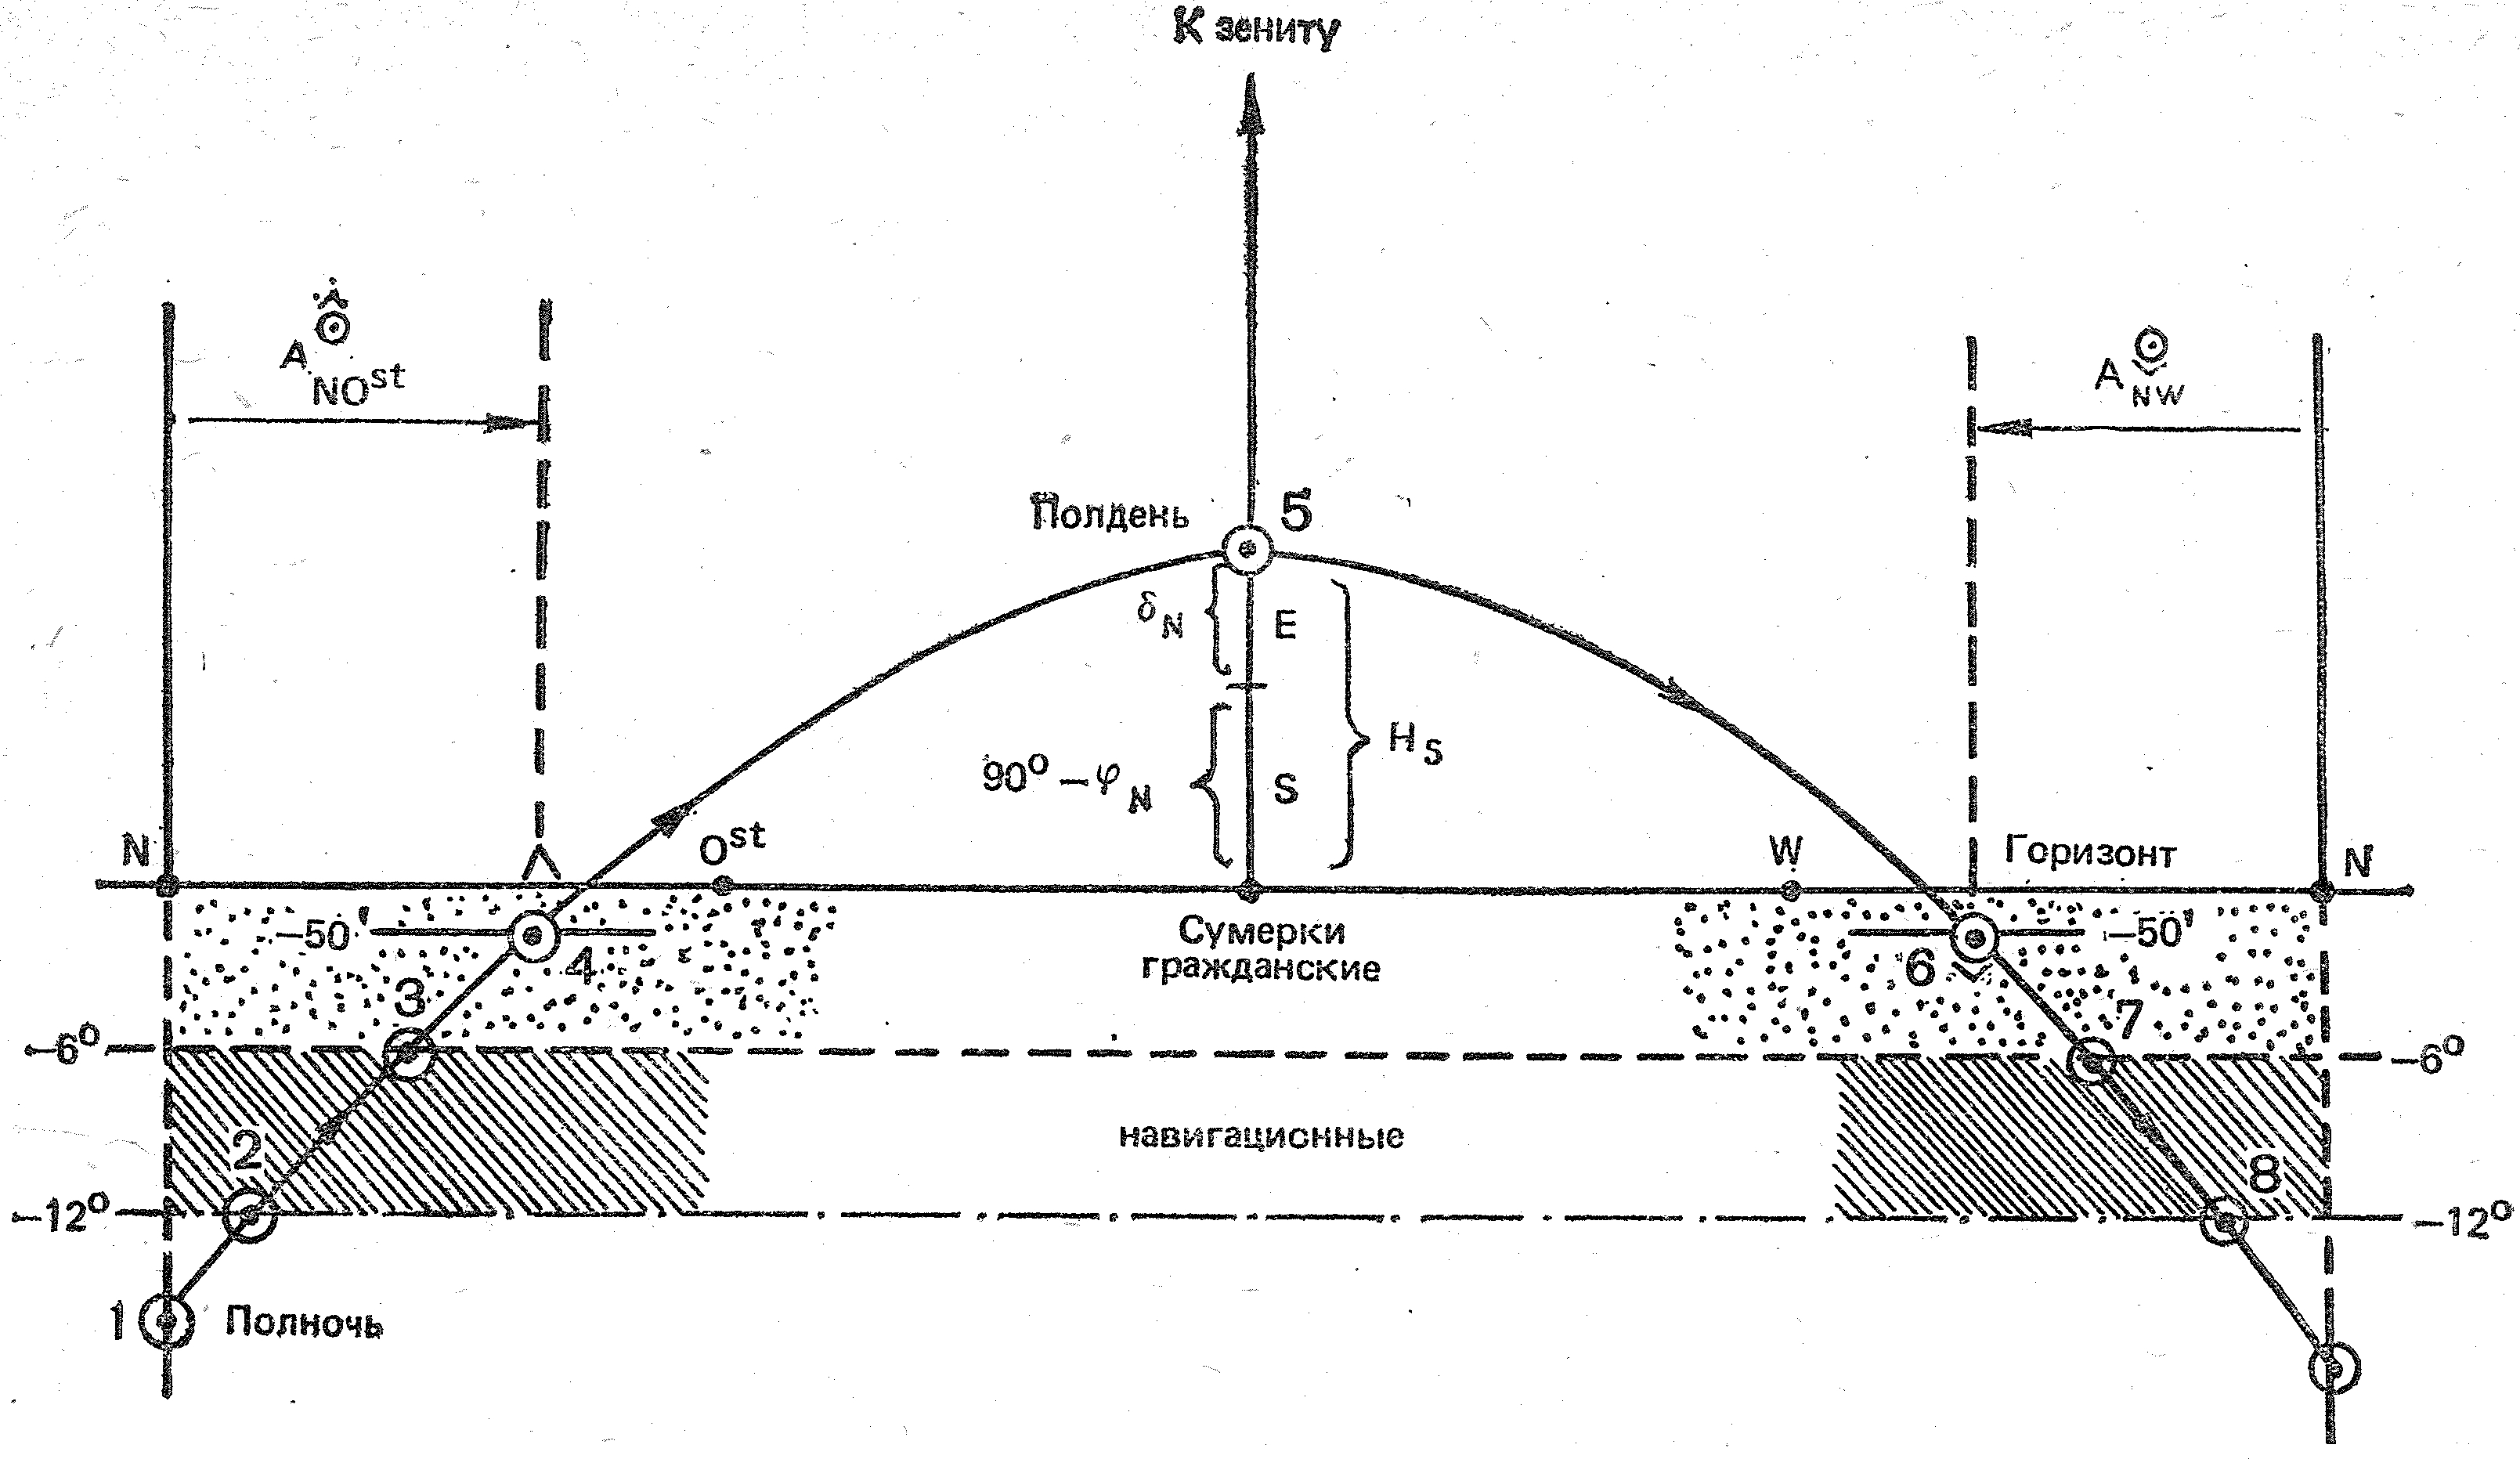
\includegraphics[width=0.8\linewidth]{0093P}
  \caption{Естественная солнечная освещенность в течение суток}
  \label{fig:93}
\end{figure*}

С приходом Солнца на снижение $-6\gr$ светает настолько, что звезды
перестают быть видимыми невооруженным глазом \--- заканчиваются
навигационные и начинаются утренние \textbf{гражданские сумерки}, которые
длятся до \textbf{восхода верхнего края} Солнца (наблюдается при снижении
Солнца около $-50'$ от уровня моря). В оптику секстана навигационные
звезды видны и в начале гражданских сумерек, поэтому данные измерения
высот звезд при ясном горизонте наиболее точны, если выполняются в
непосредственной близости к моменту окончания навигационных и начала
утренних гражданских сумерек.

В полдень (точка 5) Солнце достигает наибольшей высоты
$H = (90\gr - \varphi_N) \pm \delta^N_S$, освещенность
максимальна. Вечером после захода верхнего края Солнца (в точке 6)
наступают вечерние гражданские сумерки; они заканчиваются при снижении
Солнца на $-6\gr$, и начинают \textbf{вечерние навигационные сумерки}. Вечерние
наблюдения звезд навигационным секстаном возможны до его снижения на
$-12\gr$ (точка 8), но лучше всего их делать вблизи конца гражданских
и начала вечерних навигационных сумерек (точка 7).

Моменты судового времени восхода и захода Солнца вычисляют по МАЕ и
МТ-75; моменты наступления сумерек вычисляют по МАЕ.

\textbf{Лунная освещенность.} При астронавигационных наблюдениях
лунная освещенность учитывается как фактор, позволяющий измерять
высоты звезд в ночное время. Она определяется возрастом Луны
(см.~\ref{sec:7-1}) и оптимальна при высоте 10\otdo 40\gr в периоды
между квадратурами и полнолунием. Полная оценка лунной освещенности
производится по МАЕ, приближенное представление о ней можно составить
по формуле (\ref{eq:58}) и рис.~\ris{89}.

Оценивать астронавигационную обстановку (освещенность горизонта и
видимость светил, их расположение на небосводе) лучше всего при
подготовке к плаванию, тогда в море потребуется лишь незначительное ее
уточнение применительно к конкретному месту и времени наблюдений.

\section{Определение направления движения яхты и поправки компаса по наблюдениям светила\label{sec:7-4}}

В главе \ref{chap:6} говорилось, что направление движения яхты
определяется путевым углом \PU, который находят с учетом истинного
курса яхты \IK и угла сноса $c$. Истинный курс, в свою очередь, можно
определить по компасному курсу и поправке компаса:
$\IK = \KK + \Delta K$.

В отсутствие компаса \IK можно определить по известному истинному
пеленгу светила и курсовому углу светила \KU: $\IK = \IP \pm \KU$ (\KU
левого борта прибавляется, \KU правого борта вычитается).

В открытом море единственный способ определения поправки компаса \---
астрономический, так же как и единственный путь для ориентирования по
направлению движения (без компаса), \--- это курсоуказание
относительно направления на наблюдаемое светило, с последующим
вычислением \IK по \KU и \IP светила. Режим <<открытого моря>> в
прибрежном плавании часто создается из-за потери из видимости
береговых ориентиров при ухудшении горизонтальной видимости и т.\=,п.

\textbf{Ориентирование относительно направления на
  \starName{Полярную}.} \starName{Полярная} \--- лучший объект для
ориентирования по направлению (см. рис.~\ris{87}), так как ее истинный
пеленг находится достаточно точно при самом приближенном представлении
о месте яхты и времени наблюдений.

\IP \starName{Полярной} легко определяется по наблюдаемому на небе
расположению созвездий Кассиопеи или Большой Медведицы, так как
\starName{Полярная} удалена от Северного полюса мира $P_N$ на 1\gr в
сторону звезды $\upvarepsilon$~Кассиопеи (противоположно направлению
на $\upeta$~Большой Медведицы). Если $\upvarepsilon$~Кассиопеи или
\starName{Бенетнаш} наблюдаются на одной вертикали (в одной
вертикальной плоскости) с \starName{Полярной}, то ее
$\IP = 0\gr = 360\gr$. Если Кассиопея наблюдается слева от
\starName{Полярной} (рис.~\ris{94}, \textit{а}), то приближенно можно
принять \IP \starName{Полярной} = 359\gr при широте места менее 50\gr
или \IP \starName{Полярной} = 358\gr при широте места от 50\gr до
65\gr. Если \starName{Бенетнаш} наблюдается слева от
\starName{Полярной}, то \IP \starName{Полярной} соответственно широте
места равен 1\gr или 2\gr (рис.~\ris{94}, \textit{б}).

\begin{figure*}[!htb]
  \centering
  \includegraphics[width=\linewidth]{0094P}
  \caption{Истинный пеленг \starName{Полярной} по расположению
    созвездий Кассиопеи и Большой Медведицы относительно горизонта}
  \label{fig:94}
\end{figure*}

Более точно и в любой момент наблюдений \IP \starName{Полярной} получается из
прилож.~\ref{app:4}, \textit{г} входом по широте места (или по высоте
\starName{Полярной}) и по звездному времени \tauAries, которое может быть
вычислено по приложению~\ref{app:4}, \textit{в} или~\ref{app:4},
\textit{д} (см. примеры 7 и 9) или же получено непосредственно
глазомерной оценкой часового угла \starName{Кафф} или \starName{Фекда}
(см.~\ref{sec:7-2} и пример 8).

Измерив КП \starName{Полярной} и вычислив ее \IP на момент измерения,
можно найти поправку компаса: $\Delta K = \IP - \KP$. Если
непосредственное пеленгование звезды с компаса невозможно, то с
несколько меньшей точностью получается при одновременном измерении
курсового угла звезды и компасного курса: $\KP = \KK \pm \KU$.

Найденная величина $\Delta K$ полезна не только для контроля
правильного курсоуказания. Если на показания магнитного компаса не
влияет близко расположенное железо или магнитная буря, то
\textbf{поправка компаса должна быть равна найденному по морской карте
  магнитному склонению в данной местности}. Нарушение этого равенства
является одним из признаков неверного знания координат места
наблюдений.

В отсутствие компаса курсоуказание по \starName{Полярной}
осуществляется приведением ее на курсовой угол, при котором яхта
пойдет по намеченному пути: $\KU = \IP - (\PU - c)$. После приведения
\starName{Полярной} на вычисленный \KU, удобно заметить какое-либо
яркое светило, наблюдаемое на малой высоте по носу яхты, и править по
\KU на это светило. С течением времени направления на светила
изменяются; изменение же \IP \starName{Полярной} мал\'{о} и легко
определяется по прилож.~\ref{app:4}, \textit{г}. Курсовой угол
вспомогательного светила, наблюдаемого по носу, необходимо уточнять по
мере надобности.

\begin{table*}
  \small
  \centering
  Таблица к примеру 9: \\
  \begin{tabular}{p{0.4\linewidth}|c|c}
    \toprule
    1. Судовое время измерения компасного пеленга & $T_C$ & сентябрь, 20 \hhmm{04}{52} \\
    \midrule
    2. Часовой пояс на яхте & $\pm \mathNo^\Ost_{C_W}$ & $4$ \Ost \\
    \midrule
    3. Всемирное время $(\ppp3 = \ppp1 \mp \ppp2)$ & \Tgr & сентябрь, 20 \hhmm{00}{52} \\
    \midrule
    4. Долгота места. & $\lambda^\Ost_W$ & \hhmm{1}{08} \\
    \midrule
    5. Меридианное время $(\ppp5 = \ppp3 \pm \ppp4)$ & $T_M$ & сентябрь, 20 \hhmm{02}{00} \\
    \midrule
    6. Вспомогательная величина. & $R$ & 12\tmin \\
    \midrule
    7. Звездное время $(\ppp7 = \ppp5 - \ppp6)$ & \tauAries & \hhmm{01}{48} \\
    \midrule
    8. ИП Полярной из прилож.~\ref{app:4}, \textit{г} & \IP & $360,1\gr = 0,1\gr$ \\
    \bottomrule
  \end{tabular}
\end{table*}

\begin{small}
  \textbf{Пример 9.} 20 сентября в момент по судовому времени
  $T_C = \hhmm{04}{52}$ наблюдали звездное небо в виде показанного на
  рис.~\ris{87}. Место яхты: $\varphi = \grmm{58}{05}N$,
  $\lambda = \grmm{17}{02}\Ost$. Часы установлены по летнему московскому
  времени, $\mathNo_C = 4 \Ost$. Измерили компасный пеленг \starName{Полярной}
  $\KP = 3,0\gr$. Требуется:

  \begin{enumerate}
  \item Определить поправку компаса.
  \item Вычислить \KU, на который в отсутствие компаса следует привести
    \starName{Полярную}, если задан $\PU = 60\gr$ и угол сноса $c = +8\gr$.
  \end{enumerate}

  Решение:
  \begin{enumerate}
    \itemОпределение \IP \starName{Полярной}:
      \begin{itemize}
      \item глазомерно: так как $\upvarepsilon$~Кассиопеи (или
        \starName{Бенетнаш}) видна на одной вертикали с Полярной, то ее
        $\IP = 0\gr$;
      \item при определении звездного времени по \starName{Кафф} (или
        \starName{Фекде}):
        часовой угол \starName{Кафф} $ t_M = 2\thr = 30\gr = \tauAries$;
        часовой угол \starName{Фекда} $ t_M = 210\gr$; $\tauAries = 210\gr - 180\gr = 30\gr$.
        
        Из прилож.\ref{app:4}, \textit{г} по широте места и \tauAries: $\IP = 360,1\gr = 0,1\gr$;
      \item при вычислении звездного времени с помощью приложения~\ref{app:4},~\textit{е}.
      \end{itemize}
      Пояснения к расчетам даны в примерах~1, 3, в~\ref{sec:7-2} для
      действий 1\==3.  При действии~4 долгота места переводится в
      часовую меру по прилож.\ref{app:4},~\textit{б} с округлением до
      целой минуты.  В действии 6 \--- суточное изменение $R$ умножено
      на интервал времени (23~сентября $-$~20~сентября) и с учетом
      данных нижней шкалы взято $R = 12\tmin = 4\tmin \cdot 3$.
      
      \textbf{Примечание.} Звездное время с очень высокой точностью
      может быть вычислено по МАЕ или по
      прил.~\ref{app:4},~\textit{д}, но при ориентировании по Полярной
      этого не требуется (см. пример~12).
    \item Вычисление поправки компаса: $\Delta K = \IP - \KP = 0,1\gr - 3,0\gr = -2,9\gr $.
    \item Вычисление \KU \starName{Полярной} для курсоуказания
      (пренебрегая долями градуса, несущественными для навигации на яхте):
      $\KU = 0\gr - [60\gr - (+8\gr)] = -52\gr$ (левого борта).
\end{enumerate}
Схема решения этого примера понятна из рис.~\ris{87}.
\end{small}

\textbf{Ориентирование относительно направления на звезду или Солнце.}
Хорошая штурманская практика предполагает систематический контроль за
поправкой компаса и правильностью текущего курсоуказания. Поправку
компаса рекомендуется определять после поворота на новый курс и каждый
раз при смене вахты. Для ориентирования по направлению движения и
определения поправки компаса можно наблюдать любое светило (например,
звезду $\upalpha$~Близнецов \--- см. \rris{87}).

\begin{figure*}[!htb]
  \centering
  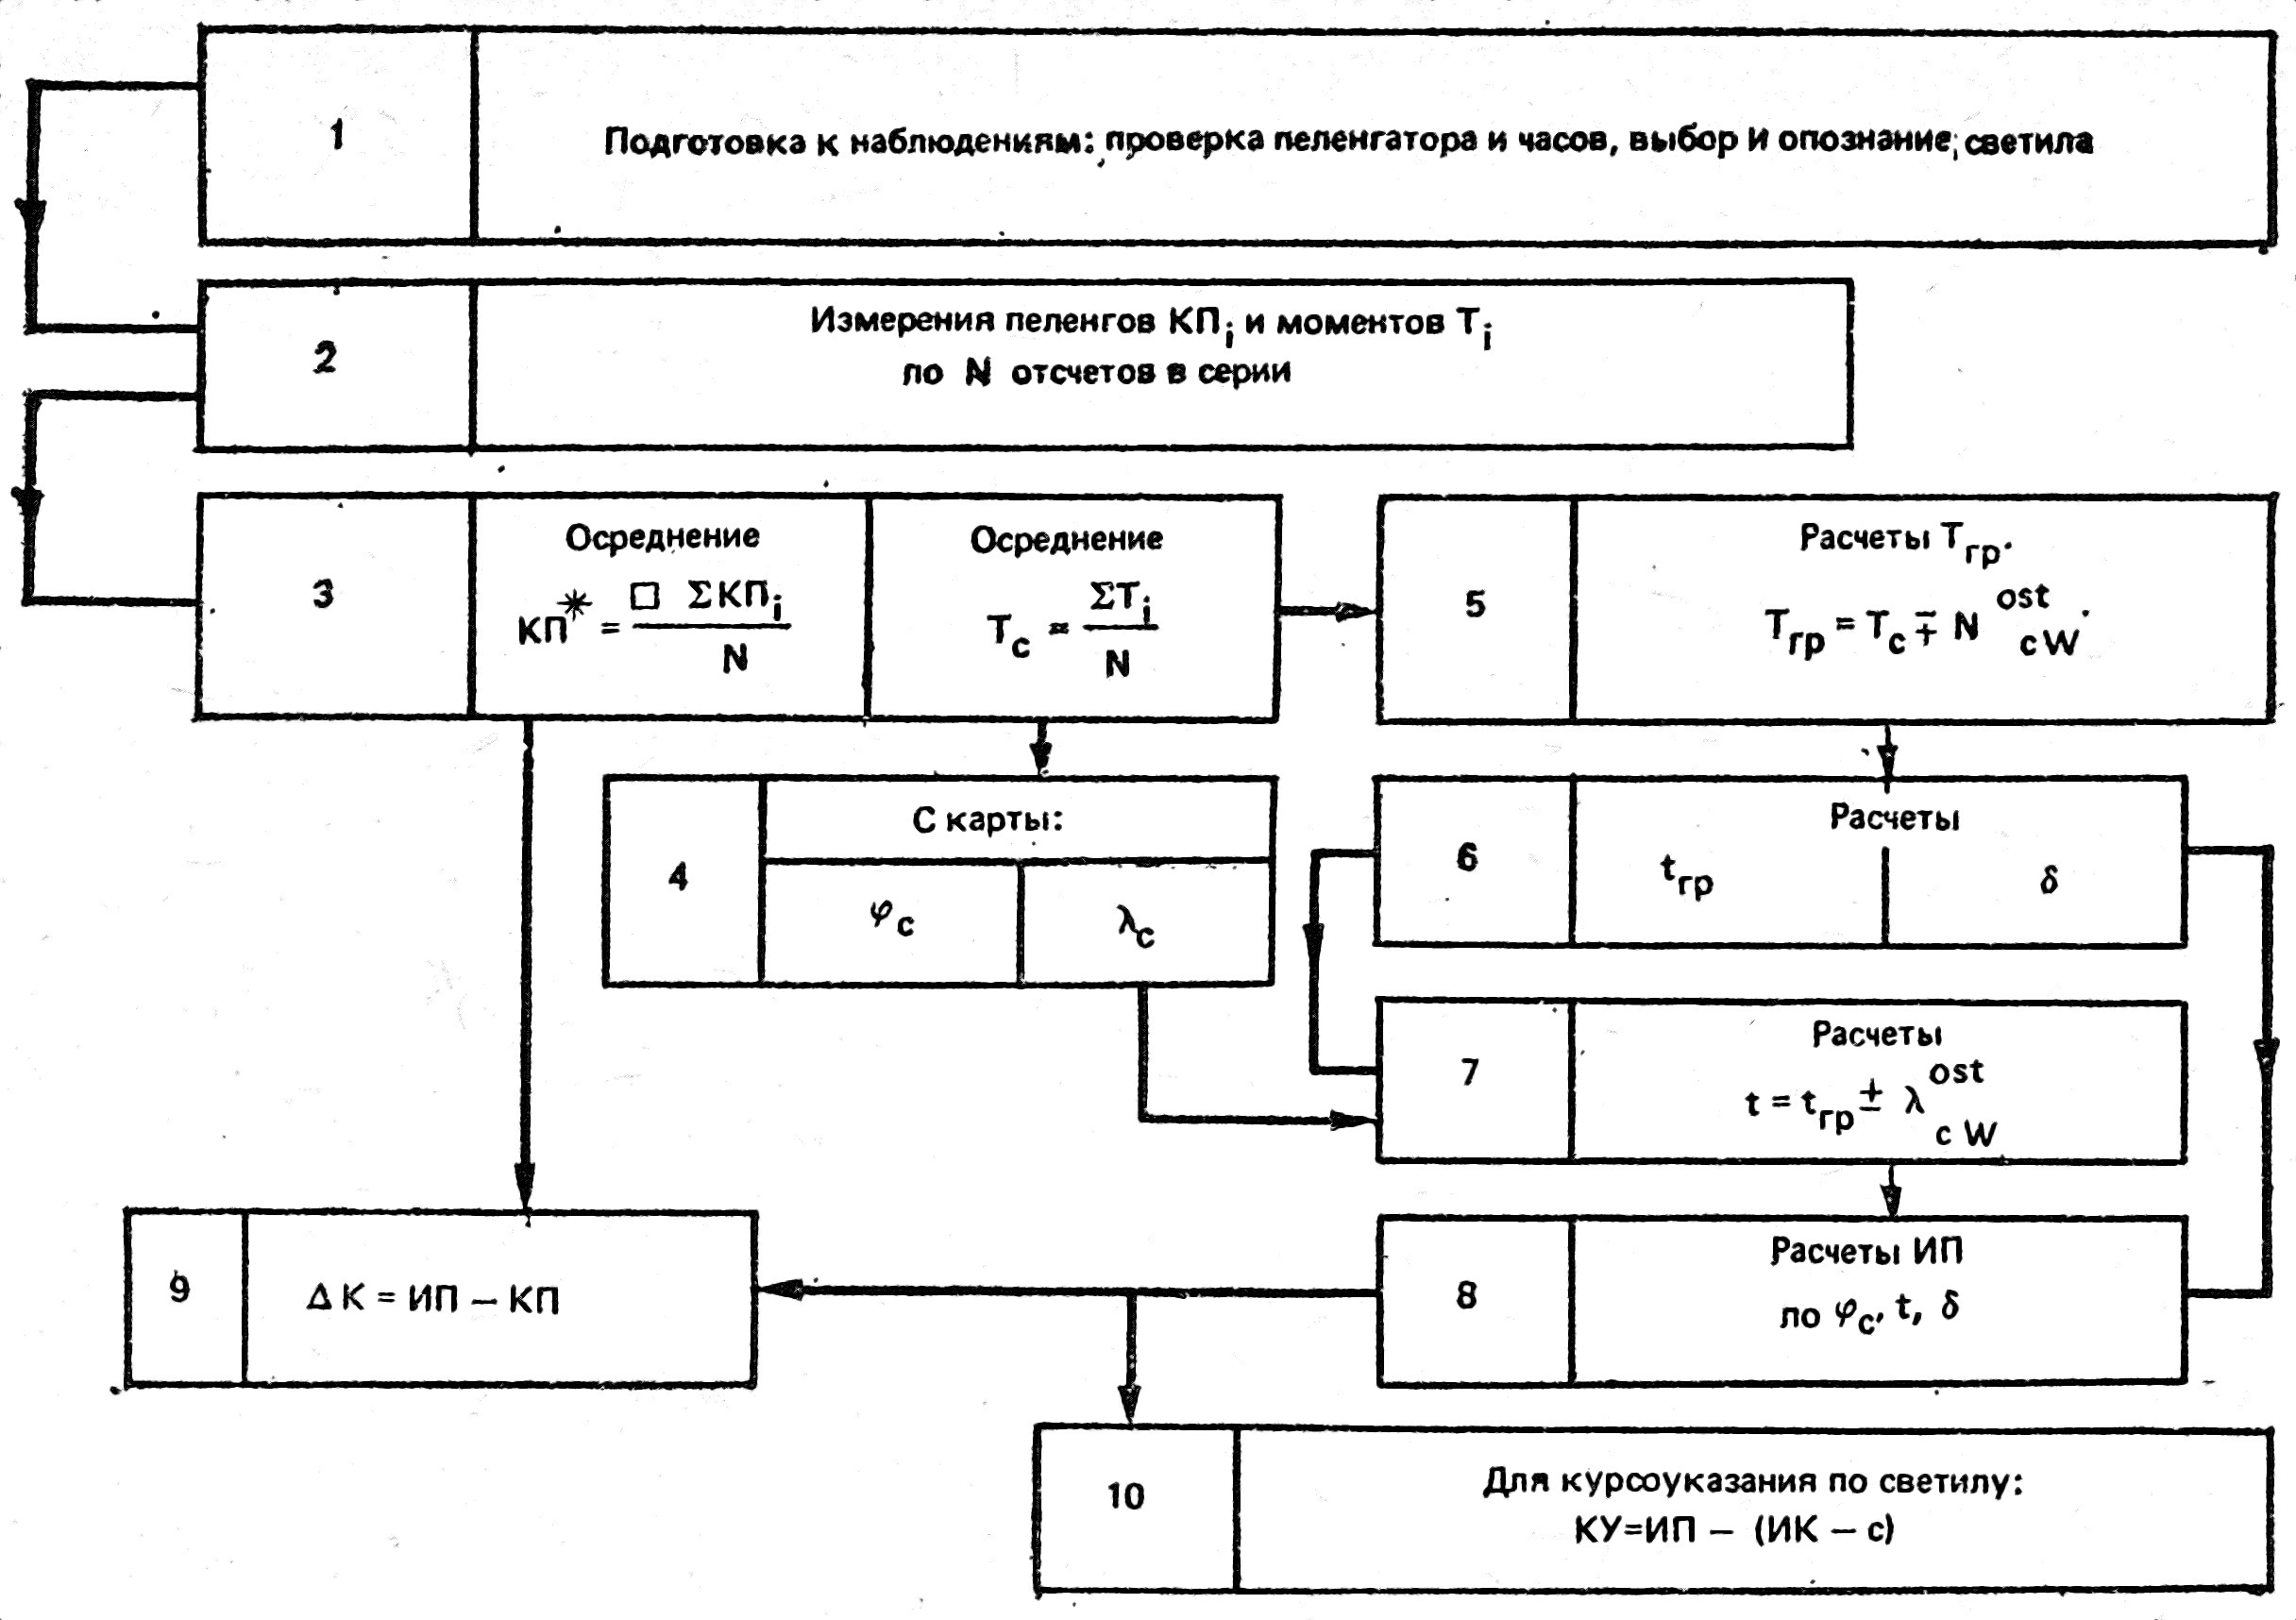
\includegraphics[width=\linewidth]{0095P.png}
  \caption{Структурно-формульная схема курсоуказания по светилу и определения поправки компаса}
  \label{fig:95}
\end{figure*}

Порядок действий при определении поправки компаса по наблюдениям
любого светила показан на \rris{95}. Поясним эту работу:

1. При подготовке к наблюдениям следует проверить пеленгатор компаса и
показания рабочих часов \--- они должны быть установлены по точному
судовому или всемирному времени с погрешностью не более $0,1\tmin$
(см. раздел~\ref{sec:7-2}). Опознав наблюдаемые светила, выберите из них
наиболее выгодное для пеленгования \--- оно должно быть хорошо видно от
компаса и иметь малую высоту: \textbf{чем меньше высота светила, тем точнее
получается поправка компаса}. Хорошо наблюдать то светило, которое
непосредственно видно через предметную мишень пеленгатора (без помощи
откидного зеркала).

2. Одновременно регистрируют компасный пеленг светила $\KP_i$, и
момент по часам $T_i$ (с точностью до $0,2\tmin$). При измерении
пеленга необходимо со всей возможной точностью удерживать котелок
компаса в горизонтальной плоскости и, наведя нить пеленгатора на
звезду или центр диска Солнца, немедленно произвести точный отсчет
$\KP_i$ и записать его. Сразу после записи КПi записать показание
часов, отбросив $0,1$\==$0,2\tmin$ (потраченные на запись \KP). При
работе с помощником по команде наблюдателя <<Ноль!>> в момент измерения
$\KP_i$ помощник регистрирует и записывает показание часов $T_i$, а затем
продиктованный наблюдателем отсчет $\KP_i$. Для компенсации случайных
погрешностей принято измерять серию пеленгов и моментов.

3. Расчет средних арифметических значений величин \KP и $T$. В отсутствие
пеленгатора или в случае невозможности пеленговать непосредственно по
компасу, следует одновременно регистрировать курсовой угол светила,
компасный курс и момент времени, а затем вычислять $\KP_i$ светила.

4. На средний момент пеленгования $T$ по навигационной прокладке пути
яхты находят ее координаты $\varphi_C$ и $\lambda_C$.

5-7. Вычисляют всемирное время наблюдений \Tgr, соответствующие ему
координаты географического места светила $\delta$ и \cidx{t}{ГР}, $t_M$. Детальное
пояснение этого этапа изложено в разд.~\ref{sec:7-5}.

8. По широте места наблюдений $\varphi_C$, склонению светила $\delta$ и
местному часовому углу светила $t_M$ находят истинный пеленг светила \IP.

9. Сравнив \IP и \KP, находят поправку компаса $\Delta K = \IP - \KP$,
справедливую для того компасного курса, на котором пеленговали
светило.

При плавании без компаса по \IP светила вычисляют тот \KU, на котором
следует удерживать светило для следования по заданному направлению
пути (см. пример~9). Знание этого \KU полезно и для текущего контроля
за направлением движения при курсоуказании по компасу.

На восьмом этапе работы \IP светила может быть найден с помощью
калькулятора, по таблицам ВАС-58 или по номограмме \No90199 (ее можно
получить вместе с навигационными картами в порту).

Правила расчета \IP светила с помощью таблиц ВАС-58 даны
непосредственно в их описании. Отметим только, что эти таблицы дают
азимут в полукруговом счете, и его надо будет обратить в \IP
(см. разд.~\ref{sec:7-1}).  <<Клавишный алгоритм>> и тестовую задачу
расчета \IP светила на калькуляторе рассмотрим на примере определения
поправки компаса по наблюдениям Солнца.

\begin{small}
  \textbf{Пример 10.} 13 апреля в Эгейском море для определения
  поправки компаса измерили серию \KP Солнца:
  
  \begin{tabular}{cc}
    $\KP_i$ & $T_i$ \\
    253,1\gr & \hhmm{15}{48,5} \\
    253,2\gr & \hhmm{15}{49,1} \\
    253,0\gr & \hhmm{15}{49,6} \\
    253,4\gr & \hhmm{15}{50,2} \\
    253,7\gr & \hhmm{15}{50,7}
  \end{tabular}

  $\varphi_C=\coord{38}{35,4}N$, $\lambda=\coord{25}{08,2}\Ost$, $\KK=200\gr$

  Средние: $\KP^\text{\Sun}=253,3\gr$, $T=\hhmm{15}{49,7}$.

  Судовое время \--- по 2 восточному поясу.

  По МАЕ на момент $\Tgr=\hhmm{15}{49,7} - 2\thr = \hhmm{13}{49,7}$ вычислили:
  
  $\delta^\text{\Sun} = \coord{8}{55,6}N$ и $t_M=\coord{52}{06,4}W$.


% TODO: calculator  
  
\end{small}

Для быстрого вычисления \IP светила с погрешностью до 1\gr, приемлемой
для плавания на яхте, удобна номограмма \No90199 издания ГУНиО
МО. Схема правой половины этой номограммы, применяемой в северных
широтах, и порядок действий при пользовании ею приведены в
приложении~\ref{app:4},~\textit{з}. Решение примера~10 по номограмме
дает $\IP = 252\gr$. Она особенно удобна для курсоуказания по светилу,
так как быстро и наглядно показывает изменение \IP светила с течением
времени. Помня, что каждые 4\tmin западный часовой угол возрастает
(восточный \--- уменьшается) на 1\gr, получим в рассматриваемом примере:

спустя 15\tmin  после пеленгования $t \approx 56\gr$ и $\IP=255\gr$,

спустя 30\tmin  после пеленгования $t \approx 60\gr$ и $\IP=258\gr$.

Перемена широты места и склонения влияют менее заметно и учитываются
по мере необходимости,

\textbf{Ориентирование по наблюдениям Солнца вблизи горизонта.}  Центр
Солнца находится в плоскости истинного горизонта (перпендикулярной
отвесной линии) в тот момент, когда с яхты наблюдается высота его
нижнего края над видимым в средних условиях морским горизонтом, равная
около $\coord{0}{18} \approx 0,5$ видимого диаметра Солнца. Это
явление называется истинным восходом (заходом) Солнца, азимут которого
легко получить по приложению~\ref{app:4}, \textit{е} (номограмма из
МТ-75). Входом по широте места и склонению Солнца в день наблюдений
(полученному, например, из приложения~\ref{app:4}, \textit{в})
выбирается азимут явления в полукруговом счете; ключ к номограмме
показан на рисунке.

По табл. 20, \textit{а}, \textit{б} МТ-75 таким же путем получается
полукруговой азимут восхода (захода) верхнего края Солнца на
горизонте, видимый с высоты глаза 12~м. В МТ-63 аналогичная таблица
дает азимут этого явления при наблюдениях с уровня моря.

Во всех этих случаях азимуты переводят в \IP, как это было дано в
примере~10, после чего можно приближенно определить поправку компаса
по наблюденному \KP восхода (захода).

Этот способ применяют при плавании в малых и умеренных широтах, но
наблюдениям часто препятствует плохая видимость горизонта.

Если от восхода и до захода Солнца широта места изменяется
незначительно, то, измерив компасный пеленг видимого восхода $\KP^{\SunriseA}$ и
видимого захода $\KP^{\Sunset}$ можно определить поправку компаса, не пользуясь
никакими пособиями (см. рис.~\ris{93} и~\ris{96}).Средний пеленг, вычисленный по
двум имеющимся, равен компасному пеленгу истинной точки юга $S$,
поэтому:

\begin{equation}
  \label{eq:71}
  \Delta K = 180\gr - \frac{\KP^{\SunriseA} + \KP^{\Sunset}}{2}
\end{equation}

\begin{figure}[!htb]
  \centering
  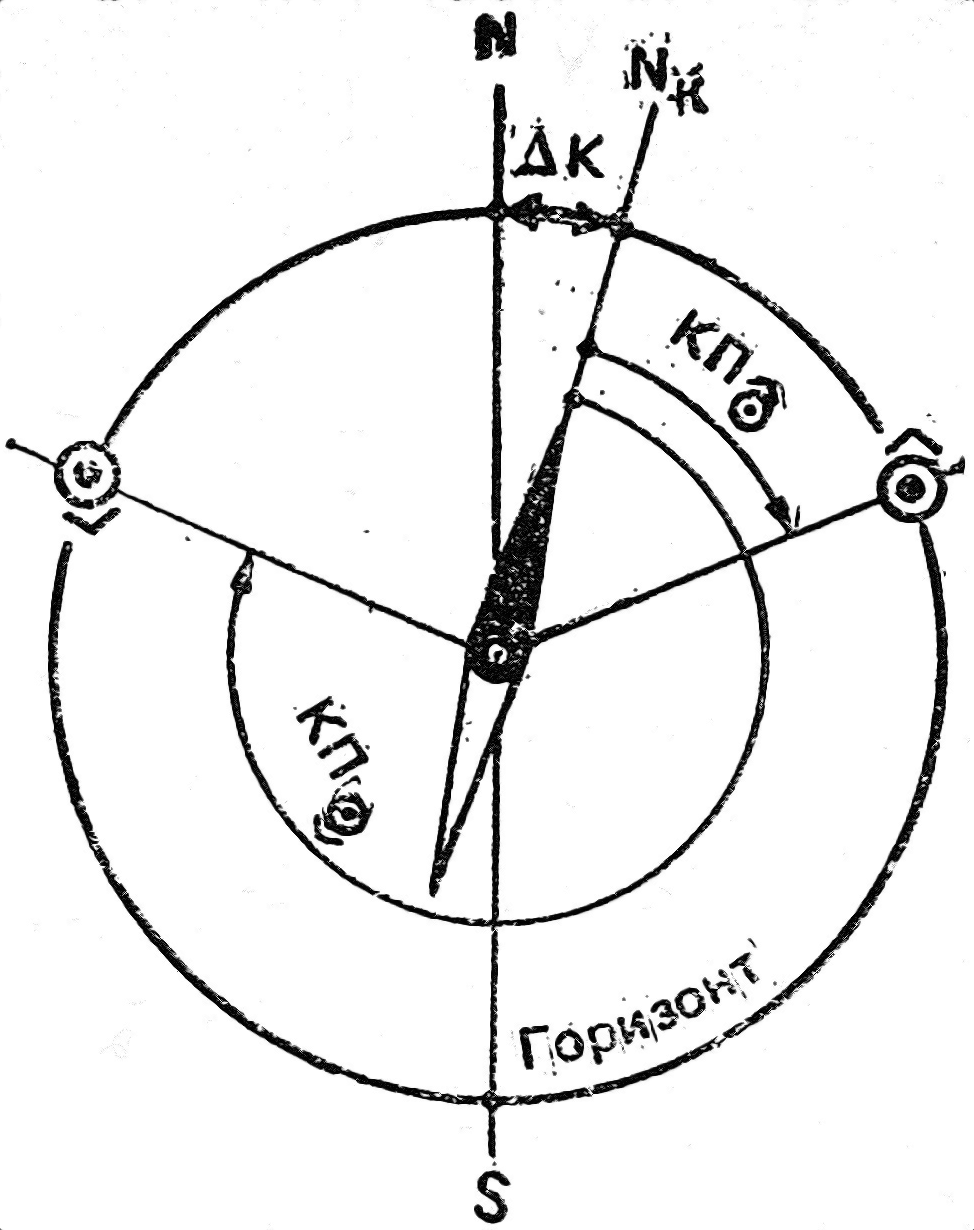
\includegraphics[width=\linewidth]{0096P.png}
  \caption{Определение поправки компаса по пеленгам восхода и захода Солнца}
  \label{fig:96}
\end{figure}

При наличии секстана направление на юг может быть приближённо
определено по наступлению наибольшей наблюдаемой высоты Солнца
(соответствует моменту наступления кратчайшей тени от вертикально
установленного шеста). Направление на точки востока и запада может
быть приближенно определено по приходу Солнца на высоту, указанную в
табл. 21 (МТ-75), либо по восходу и заходу звезды \deltaStar{Ориона}
(верхняя в <<поясе Ориона>>). Изложенные правила и рекомендации
ориентирования по наблюдениям направлений на светила даны в
предположении плавания в северных широтах выше параллели $23,5\gr N$.

\section{Ориентирование по местонахождению\label{sec:7-5}}

Астронавигационные способы определения места доступны в любом районе
плавания и в любое время суток, если по метеорологическим условиям
светила можно наблюдать, а другие способы исключаются
обстановкой. Астронавигационные способы обсервации проверены вековой
практикой мореплавания. Во многих случаях они дают наиболее точный
результат, а часто являются единственно возможными способами контроля
счисления пути.

\textbf{Принцип определения географического места яхты по наблюдениям
  светил.}  Предположим, что яхта находится в точке $M$ Атлантического
океана (\rris{97}) и на морской карте это место изображается в точке
$M$ (\rris{98}).  Отвесная линия в месте нахождения яхты имеет
направление $OM$ \--- на яхте его можно указать с помощью отвеса (груза,
подвешенного на нити) или относительно направления на горизонт, так
как плоскость горизонта \textit{Г} всегда перпендикулярна отвесной линии.

\begin{figure}[!htb]
  \centering
  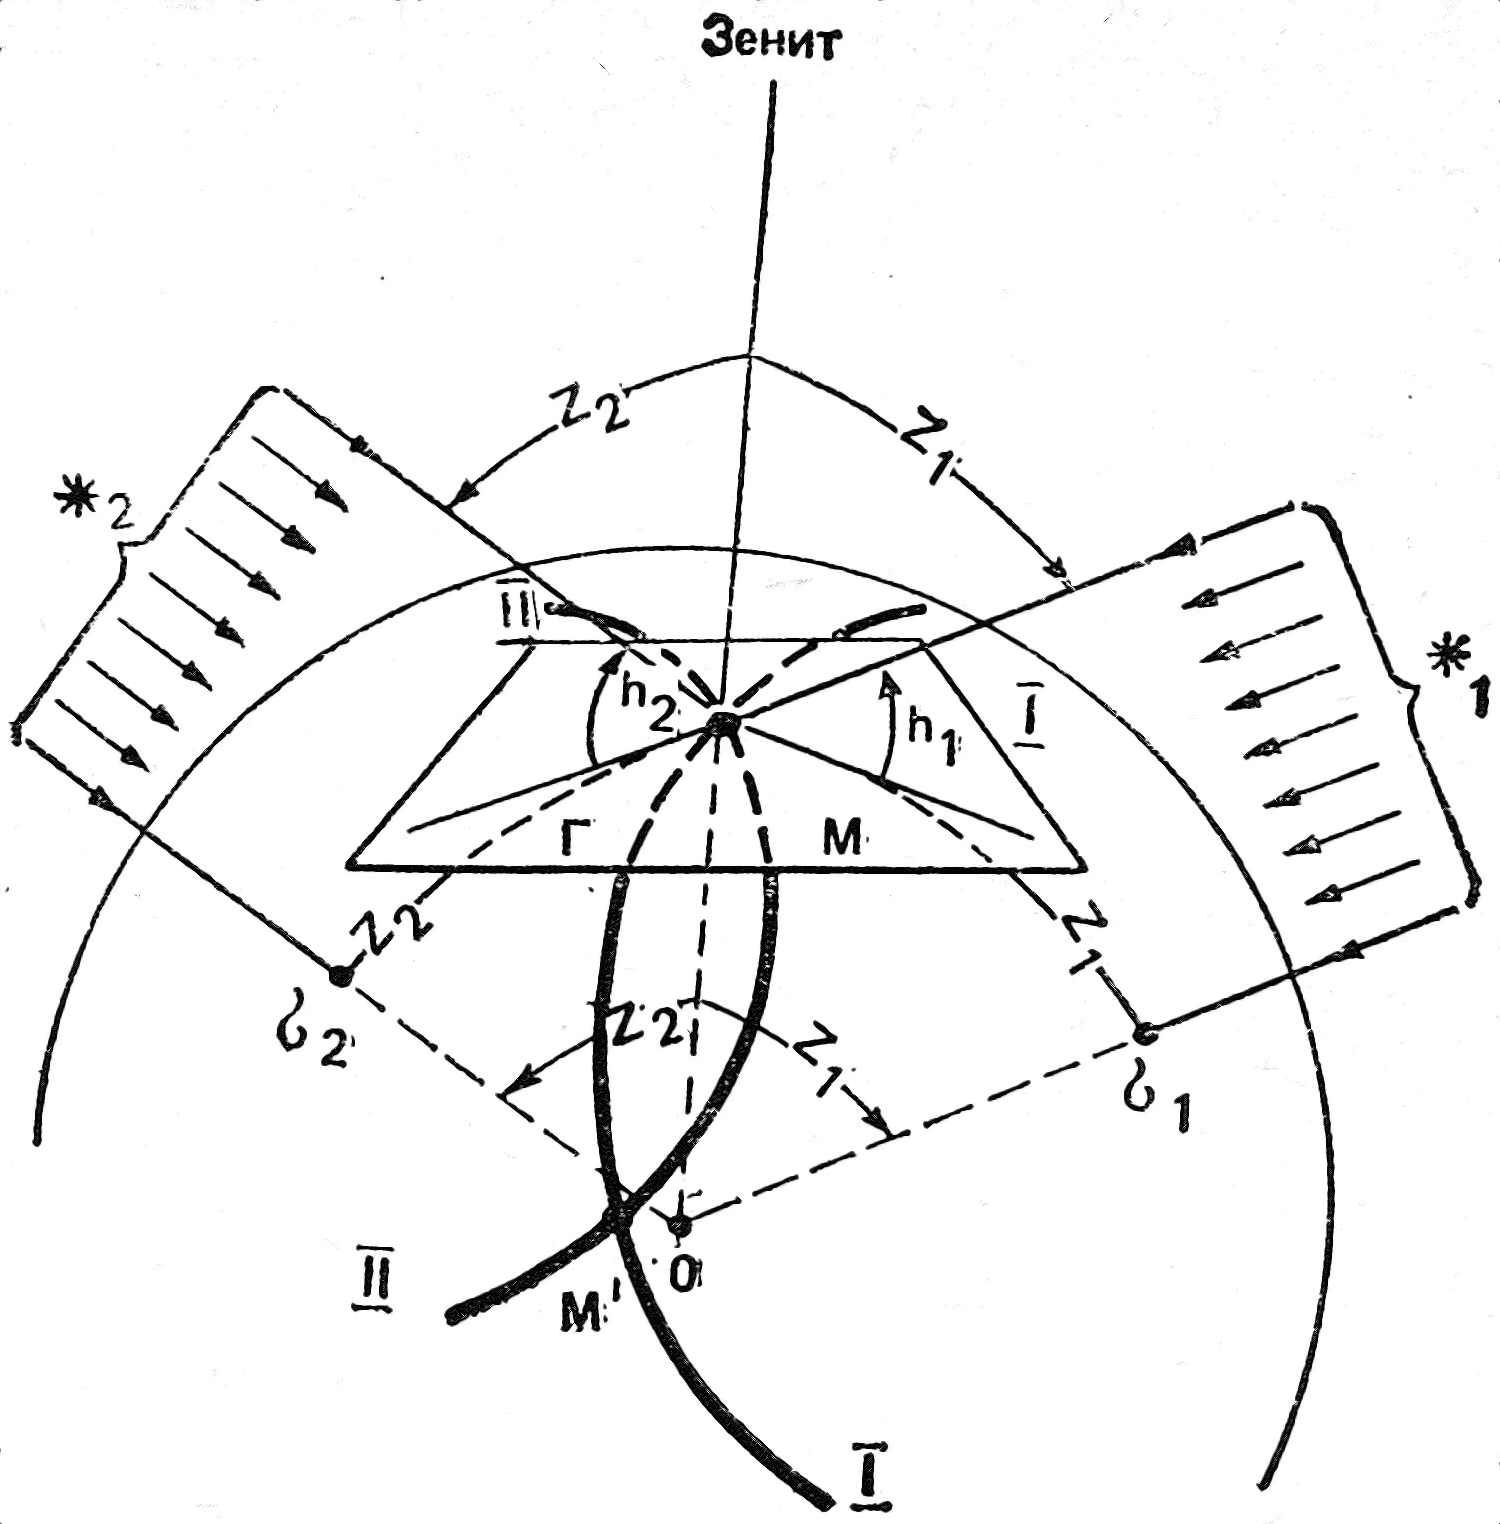
\includegraphics[width=\linewidth]{0097P.png}
  \caption[Астронавигационное место яхты]{Астронавигационное место яхты определяется точкой пересечения кругов равных высот I-I и II-II на поверхности Земли}
  \label{fig:97}
\end{figure}

\begin{figure*}[!htb]
  \centering
  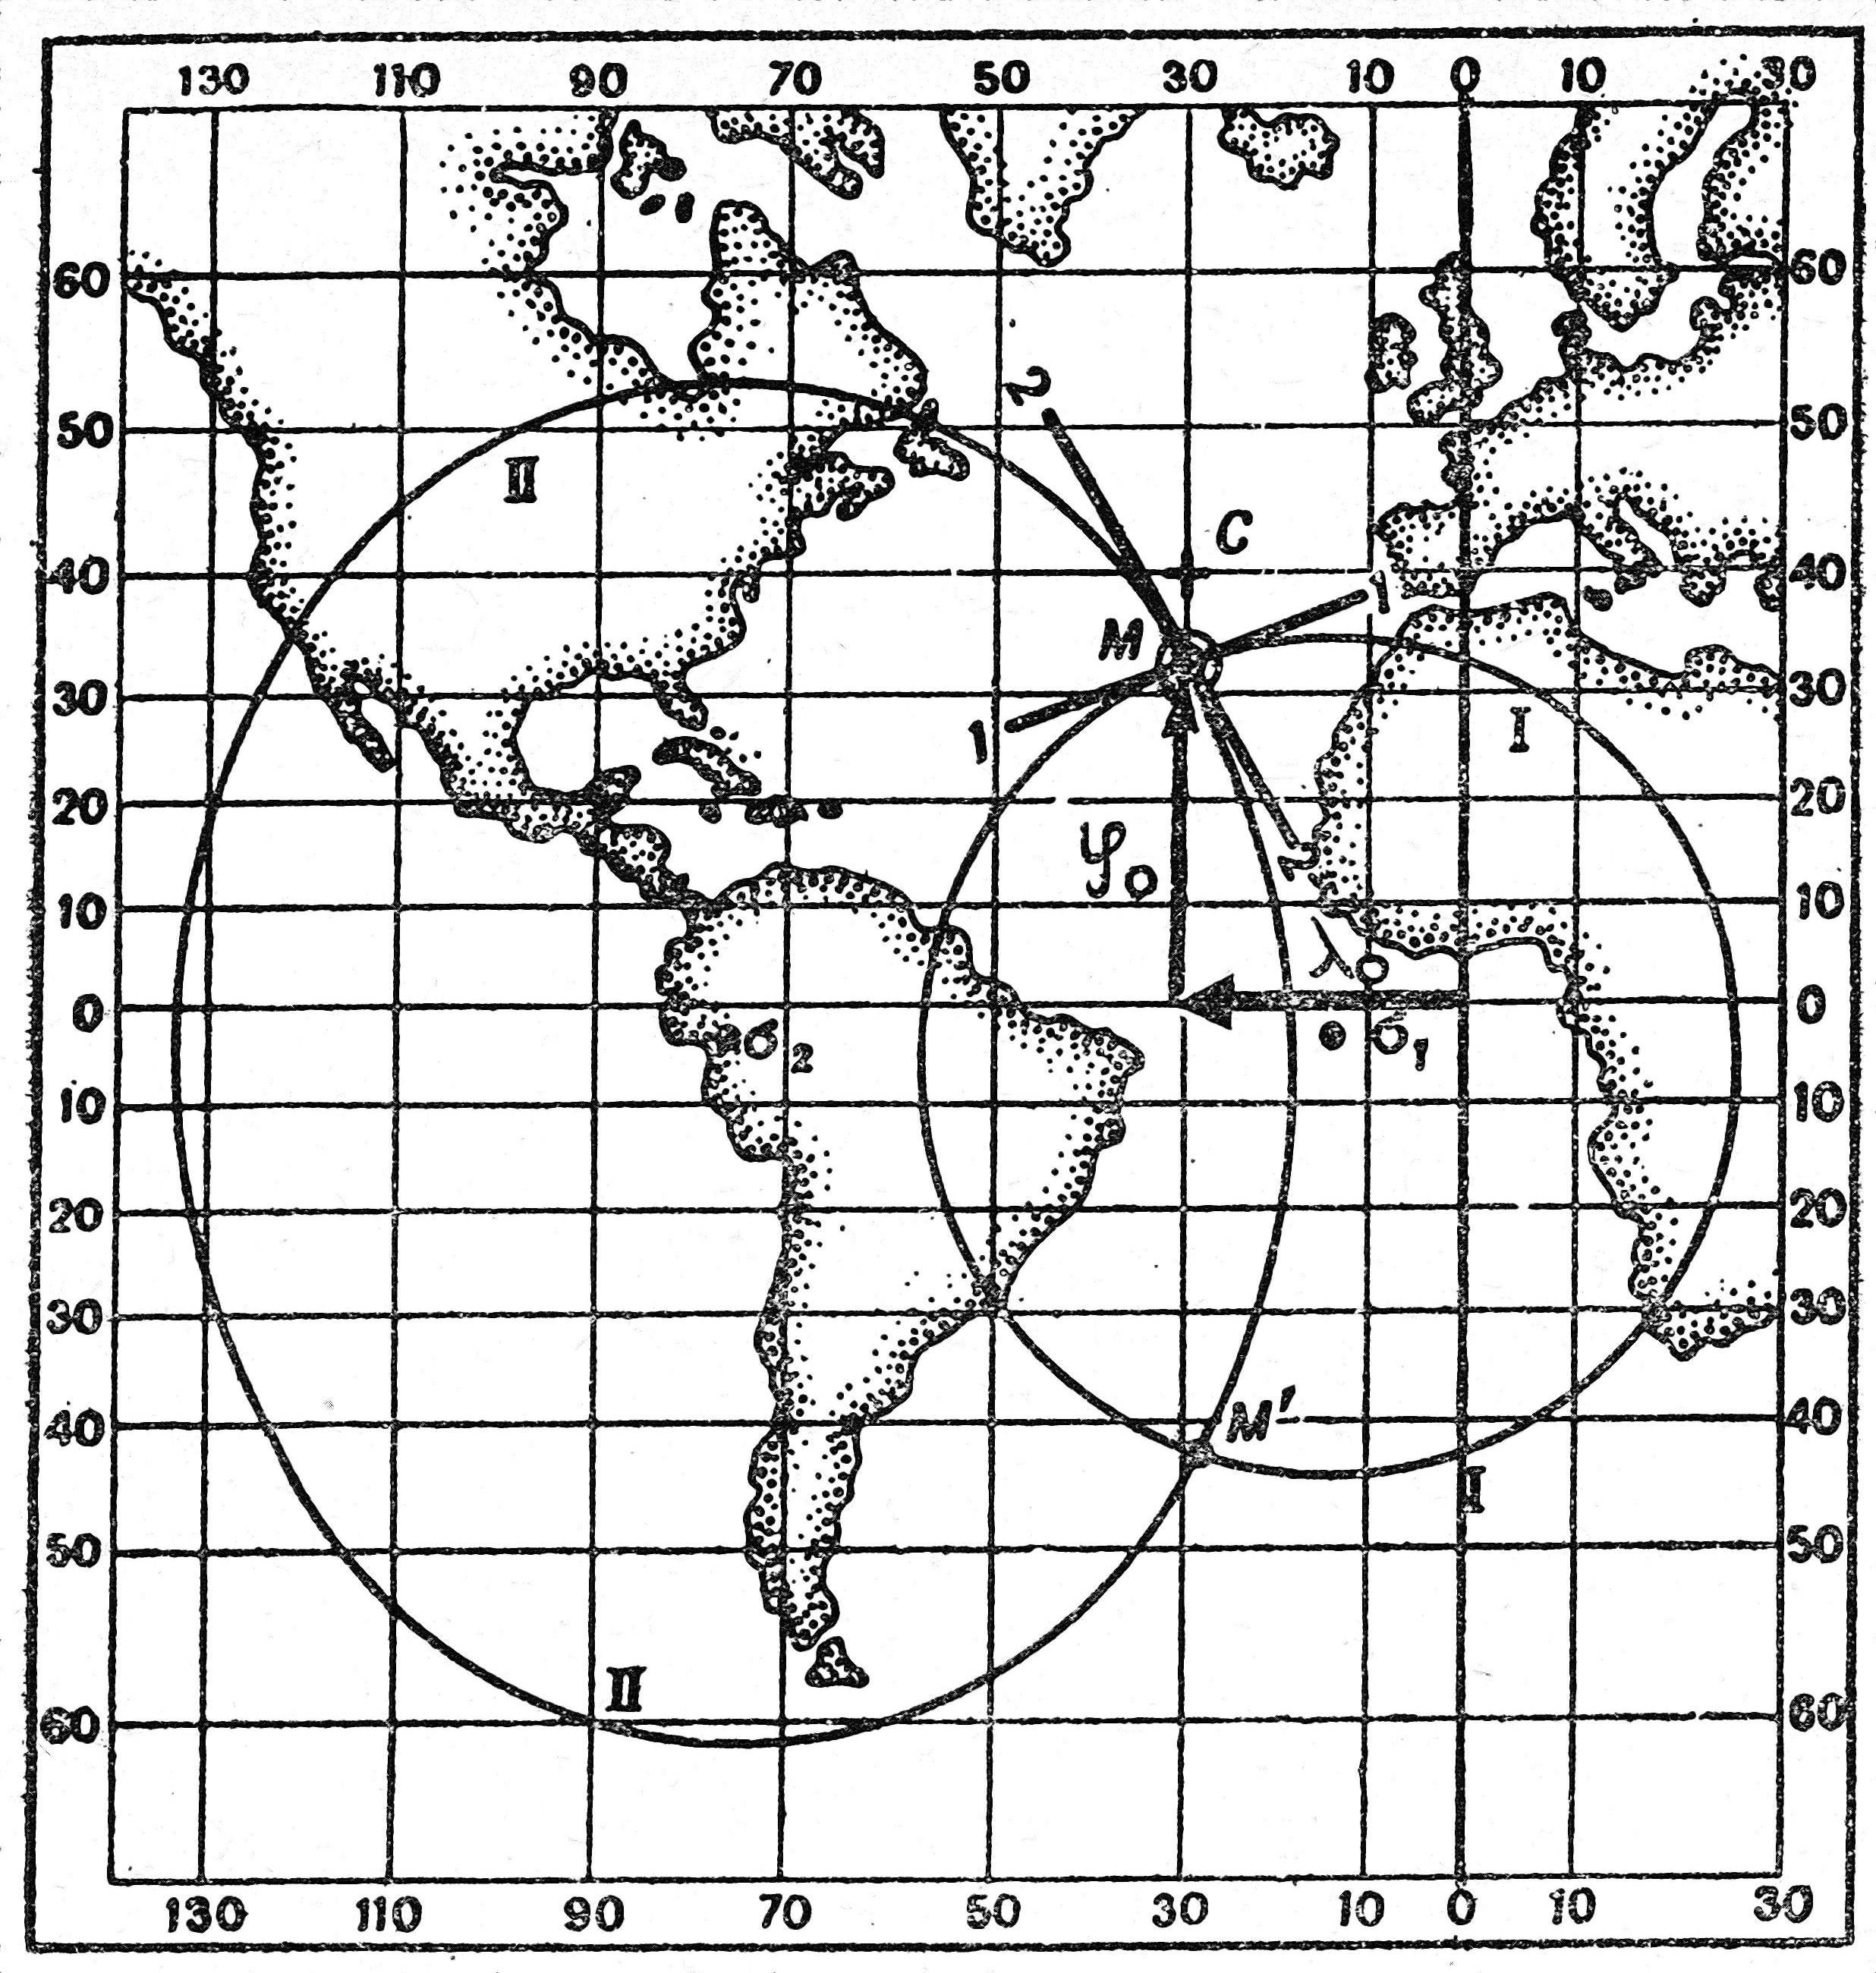
\includegraphics[width=0.8\linewidth]{0098P.png}
  \caption[Круги равных высот на морской карте]{На морской карте круги равных высот \--- сложные кривые, их заменяют высотными линиями положения 1-1 и 2-2}
  \label{fig:98}
\end{figure*}

По определению географических координат (см. гл.~\ref{chap:6}) видно,
что они изменяются вследствие изменения направления отвесной линии при
перемещении из одного места на Земле в другое: плоскость меридиана
места всегда проходит через ось вращения Земли и отвесную линию в
данном месте, широта указывает угол $\varphi_0$ между плоскостью
экватора и направлением отвесной линии, долгота $\lambda_0$ определяет
положение меридиана места относительно начального (Гринвичского)
меридиана. Поэтому для определения географического места яхты достаточно
найти направление отвесной линии в месте наблюдений относительно
направлений на внешние ориентиры, географическое положение которых
известно.

Если с яхты наблюдаются светила $*_1$ и $*_2$, то
можно полагать, что географические места этих светил известны \--- в
разд.~\ref{sec:7-1} было пояснено, что широта точки $\sigma_1$
тождественна склонению светила $*_1$ ($\varphi^* = \delta_1$),
а ее долгота \--- гринвичскому часовому углу светила
($\lambda^*_1 = \Tgr$) в полукруговом счете; алогично можно записать,
что $\varphi^*_2 = \delta_2$, $\lambda^*_2 = \Tgr$. Склонения и гринвичские
часовые углы светил легко получить на момент наблюдений из МАЕ или
другого пособия аналогичного назначения. Следовательно, географические
места светил $\sigma_1$ и $\sigma_2$ можно рассматривать в качестве <<маяков>> и
относительно них определить место яхты, если измерить расстояния $z_1$ и
$z_2$. Подобно навигационному определению места яхты по расстояниям до
двух маяков, астронавигационное место яхты получится в пересечении
двух окружностей, описанных радиусами $z_1$ и $z_2$ из соответствующих им
географических мест светил $\sigma_1$ и $\sigma_2$. Двойственность решения задачи
легкоразрешима; расстояние между возможными местами $M$ и $M_1$ очень
велико, и счислимое место $C$ указывает, что яхта была в точке $M$.

Расстояния $z_1$ и $z_2$ можно получить двумя путями, учитывая, что
лучи от светил, приходящие в центр Земли и на яхту,
параллельны. Расстояние $z_1$ равно длине дуги, измеряющей угол $z_1$
при центре Земли. Но этот угол равен углу между отвесной линией $Mz$ и
направлением на светило $M_{\sigma_1}$, иначе говоря \--- зенитному
расстоянию первого светила. Аналогично расстояние $z_2$ равно
зенитному расстоянию второго светила. Непосредственное измерение
зенитных расстояний $z_1$ и $z_2$ можно выполнить астролябией
(см. \rris{103}), где положение ответной линии определяется с помощью
отвеса.

В морских условиях измерения зенитных расстояний астролябией трудны и
не всегда достаточно точны. Лучший результат дает применение
навигационного секстана, которым измеряют угол между плоскостью
горизонта и направлением на светило, т.е. высоту светила $h$. По
известной высоте легко найти зенитное расстояние: $z_1 = 90\gr - h$.

Нетрудно видеть, что в любой точке окружности радиуса $z$ высота светила
одинакова, поэтому ее называют \textbf{кругом равных высот}. Круг равных высот
на морской карте отличается от окружности, кроме того, в подавляющем
большинстве случаев географические места светил не помещаются на
путевой карте. Поэтому непосредственно круги равных высот раиусами $z_1$
и $z_2$ не строят. Небольшие отрезки кругов равных высот вблизи
счислимого места полагают прямыми 1\==1 и 2\==2 (\rris{98}); их называют
\textbf{высотными линиями положения} и строят на путевых картах при
астронавигационных обсервациях.

Таким образом, для астронавигационного определения места необходимо:

\begin{itemize}
\item измерить высоты (или зенитные расстояния) светил и
  соответствующие им моменты времени;
\item вычислить координаты географических мест светил на моменты
  измерений высот;
\item построить высотные линии положения на путевой карте;
\item привести эти линии положения к одному месту наблюдений (если
  яхта в ходе наблюдений перемещалась) и найти обсервованное место, а
  также рассчитать точное судовое время обсервации;
\item сравнить результаты счисления и обсервации, принять решение о
  причинах обнаруженного сноса яхты с намеченного пути и необходимой
  корректуре навигационной прокладки.
\end{itemize}

Точность обсервации в первую очередь зависит от точности измерений
высот, а также точности их исправления поправками, компенсирующими
погрешности секстана и влияние внешней среды. Надо помнить, что
высотная линия положения очень чувствительна к погрешностям в высоте
светила. Например, погрешность в высоте на $1'$ дает смещение линии
положения от верного места яхты на 1~милю, т.е. погрешность высоты
равна погрешности линии положения.

\textbf{Измерение и исправление высоты светила.} Для измерения высоты
светила секстан устанавливают в вертикальной плоскости, проходящей
через светило $\sigma$ (\rris{99}). \textbf{Малое зеркало} (2) и
\textbf{большое зеркало} (5) секстана перпендикулярны плоскости его
рамы (3). В рабочем положении секстан удерживают \textbf{рукояткой}
(9), опирающейся на \textbf{планку} (8). Наблюдения выполняют с
помощью \textbf{ночной трубы} (7); ее поле зрения показано справа
внизу или \textbf{дневной трубы} (6), имеющей большее увеличение, но
меньшее поле зрения и перевернутое изображение.

Луч от прямовидимого в трубу горизонта \textit{Г} непосредственно
попадает в глаз наблюдателя \textit{О} (в необходимых случаях
контрастность линии горизонта улучшают \textbf{светофильтрами}
(1). Луч от светила $\sigma$ а попадает в большое зеркало, которое
разворачивают подвижной линейкой \--- \textbf{алидадой} (10) в такое
положение, при котором луч от светила пройдет к малому зеркалу и от
него \--- к глазу наблюдателя. Таким путем добиваются приближенного
сведения изображения горизонта и отраженного изображения светила в
поле зрения трубы. Отпустив стопор алидады, вращением барабана точного
отсчета (12) добиваются точного совмещения изображения светила и
горизонта при вертикальном положении рамы секстана. Отсчет высоты
получают суммированием грубого отсчета по градусной шкале лимба,
нанесенного на раме, и точного отсчета по минутной шкале на
барабане. Ночью пользуются \textbf{осветителем шкал} (11). При
наблюдениях Солнца между большим и малым зеркалами устанавливают один
из \textbf{светофильтров} (4).

При подготовке к плаванию проверяют параллельность оси трубы плоскости
рамы секстана (\rris{100},~\textit{а}) с помощью уголковых диоптров,
входящих в комплект секстана, \--- их ставят на лимб и наводят на
удаленный предмет. С помощью отвертки вращают регулировочные винты на
оправе стойки трубы и приводят горизонтальный срез предмета в середину
поля зрения.

При подготовке к морским наблюдениям проверяют с помощью диоптров
перпендикулярность большого зеркала плоскости рамы (\rris{100},~\textit{б}),
регулируя зеркало винтом, имеющимся на его тыльной стороне.

Затем наводят секстан на удаленный предмет и проверяют
перпендикулярность малого зеркала плоскости рамы (\rris{100},~\textit{в}): при
вращении барабана около нулевого отсчета отраженное изображение
предмета должно проходить точно через прямовидимое его
изображение. При необходимости положение малого зеркала исправляют
вращением винта, расположенного на его тыльной стороне у внешнего края
оправы.

При наблюдениях определяют поправку секстана и измеряют высоты
светил. Для определения поправки устанавливают отсчет 0\gr и наводят
трубу на удаленный предмет (более 1 мили) или светило. Совмещают
прямовидимое и отраженное изображен этого предмета (светила) и читают
получившийся отсчет секстана $oc_i$. Поправку секстана находят по форму,
$i = 0\gr (360\gr) - oc_i$, она может быть положительной или
отрицательной. При расстоянии до объекта, над которым измеряется
высота светила, менее 1 мили поправку секстана всегда определяют по
этому объекту.

Высоты светила измеряют в два этапа. На первом этапе изображение
светила приводят к линии горизонта для этого устанавливают отсчет
около 0\gr, наводят трубу на светило (при работе с Солнцем не следует
забывать установить светофильтры) затем опускают трубу к горизонту и
одновременно передвижением алидады в сторону больших отсчетов
улдерживают отраженное светило в поле зрения; грубо совместив
изображение светила с горизонтом, отпускают стопор алидады.


...раздел не окончен...

\onecolumn

%%% Local Variables:
%%% mode: latex
%%% TeX-master: "yacht-captain"
%%% End:
